% Note: requires package amssymb for \mathbb

\section{Collective Variable-based Calculations\footnote{ The features
described in this section were contributed by Giacomo Fiorin (ICMS,
Temple University, Philadelphia, PA, USA) and J\'er\^ome H\'enin (CNRS,
Marseille, France). Please send feedback and suggestions
to the NAMD mailing list.}}
\label{section:colvars}

In today's molecular dynamics simulations, it is often useful to
reduce the great number of degrees of freedom of a into a few
parameters which can be either analyzed individually, or manipulated
in order to alter the dynamics in a controlled manner.  These have
been called `order parameters', `collective variables', `(surrogate)
reaction coordinates', and many other terms.  In this section, the
term `collective variable' (shortened to \textit{colvar}) is used, and
it indicates any differentiable function of atomic Cartesian
coordinates, $\bm{x}_{i}$, with $i$ between $1$ and $N$, the total
number of atoms:
\begin{equation} 
  \label{eq:colvar_basic}
  \xi(t) \; = \xi\left(\bm{x}_{i}(t), \bm{x}_{j}(t), \bm{x}_{k}(t),
  \ldots \right)\;, \;\; 1 \leq i,j,k\ldots \leq N
\end{equation}

The colvars module in NAMD may be used in both MD simulation and
energy minimization runs (except free energy methods).
It offers several features:
\begin{itemize}

\item define an arbitrary number of colvars, and perform a
  multidimensional analysis or biased simulation by accessing any
  subset of colvars independently from the rest (see
  \ref{sec:colvarmodule});

\item combine different functions of Cartesian coordinates (herein
  termed colvar \emph{components}) into a colvar defined as a
  polynomial of several such components, thereby implementing new
  functional forms at runtime; periodic, multidimensional and
  symmetric components are handled transparently (see \ref{sec:cvc});

\item calculate potentials of mean force (PMFs) for any set of
  colvars, using different sampling methods: currently implemented are
  the Adaptive Biasing Force (ABF) method (see
  \ref{sec:colvarbias_abf}), metadynamics (see
  \ref{sec:colvarbias_meta}), Steered Molecular Dynamics (SMD) and
  Umbrella Sampling (US) via a flexible harmonic restraint bias (see
  \ref{sec:colvarbias_harmonic});

\item calculate statistical properties of the colvars, such as their
  running averages and standard deviations, time correlation
  functions, and multidimensional histograms, without the need to save
  very large trajectory files.

\end{itemize}


\subsection{General parameters and input/output files}
\label{sec:colvarmodule}

The structure of a typical colvars configuration is represented in
Figure~\ref{fig:colvars_diagram}.  Each colvar is a combination of one
or more \emph{components} (see \ref{sec:colvar}), which are functions
of several atomic coordinates.  Many different biasing or analysis
methods can be applied to the same colvars.  But care should be taken
that certain methods (such as free energy reconstruction) do not
produce correct results when other biases are adding forces to their
colvars.

\begin{figure}[!ht]
  \centering
  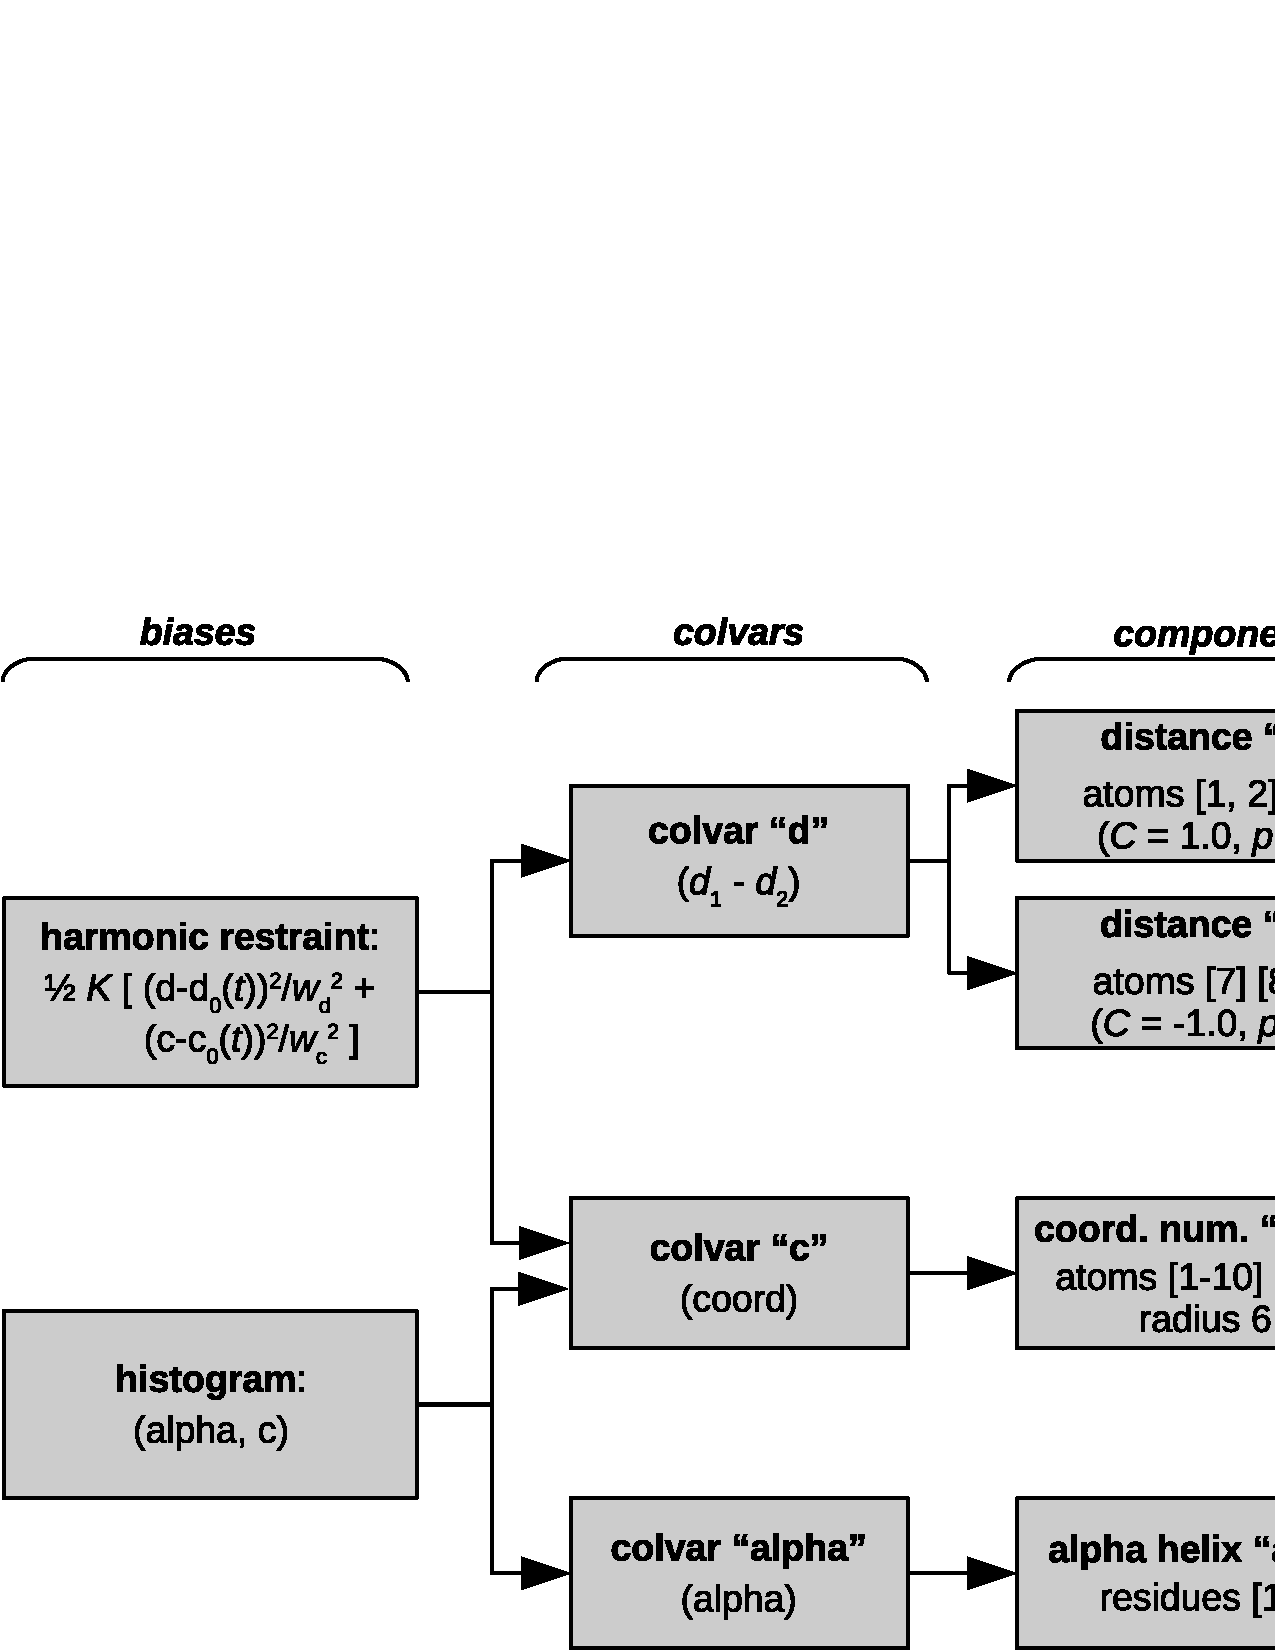
\includegraphics[width=12cm]{figures/colvars_diagram}
  \caption{Example of a collective variables (colvar) configuration.
    The colvar ``$d$'' is defined as the difference between two
    distances, each calculated between the centers of mass of two
    atom groups.  The second colvar ``$c$'' holds the coordination
    number (i.e.~the number of contacts) within a radius of 6~\AA{}
    between two groups.  The third colvar ``alpha'' measures the
    degree of $\alpha$-helicity of the protein segment between
    residues 1 and 10. A moving harmonic restraint is applied to the
    colvars ``$d$'' and ``$c$'', each rescaled by means of width
    parameters $w_{d}$ and $w_{c}$; the centers of the restraint,
    $d_0$ and $c_0$, evolve with the simulation time $t$. The joint
    histogram of ``alpha'' and ``$c$'' is also recorded on-the-fly.}
  \label{fig:colvars_diagram}
\end{figure}


\subsubsection{NAMD parameters}

To enable a colvar calculation, two parameters should be added to the
NAMD configuration file must set (three when restarting a previous
run):

\begin{itemize}
  \setlength{\itemsep}{0.4cm}

\item %
  \NAMDCONFWDEF{%
    colvars}{%
    Enable the collective variables module}{%
    boolean}{%
    \texttt{off}}{%
    If this flag is on, the collective variables module within NAMD is
    executed at each time step; the module requires a separate
    configuration file, to be provided with \texttt{colvarsConfig}.}

\item %
  \NAMDCONF{%
    colvarsConfig}{%
    Configuration file for the collective variables}{%
    UNIX filename}{%
    This file contains the definition of all collective variables and
    their biasing or analysis methods.  It is meant to contain all the
    information needed to \emph{begin} a colvars simulation.
    Additional information is needed instead to \emph{continue} a
    previous run, which is read from the file provided by
    \texttt{colvarsInput}.}

\item %
  \NAMDCONF{%
    colvarsInput}{%
    Input state file for the collective variables}{%
    UNIX filename}{%
    When continuing a previous simulation run, this file contains the
    current state of all collective variables and their biasing
    methods.  Its format is similar to that of \texttt{colvarsConfig},
    but with different keywords.  In normal circumstances, this file
    is written automatically at the end of a NAMD run, and the user
    does not need to edit it.}

\end{itemize}

\subsubsection{Output files}

By default, the collective variables module writes three output
files:
\begin{itemize}

\item a \emph{state file}, named
  \texttt{$<$outputName$>$.colvars.state}; this file is in ASCII
  format, regardless of the value of \texttt{binaryOutput} in the NAMD
  configuration; the name of this file can be provided as
  \texttt{colvarsInput} to continue the simulation in the next run;

\item a \emph{restart file} (equivalent to the state file) is written
  every \texttt{colvarsRestartFrequency} steps, if either
  \texttt{colvarsRestartFrequency} or the NAMD parameter
  \texttt{restartFreq} is defined; its name is
  \texttt{$<$restartName$>$.colvars.state}, and can be given as
  \texttt{colvarsInput} to continue an interrupted run; (provided that
  the coordinates and velocities restart files at the same time step
  are also used);

\item a \emph{trajectory file} is written during the simulation, if
  the colvars module parameter \texttt{colvarsTrajFrequency} is
  greater than 0 (default: 100); its name is
  \texttt{$<$outputName$>$.colvars.traj}; unlike the state file it is
  not needed to restart a simulation, but can be read in for
  post-processing (see~\ref{sec:colvar_acf}).

\end{itemize}

Other output files may be written by specific methods applied to the
colvars (e.g.~by the ABF method, see \ref{sec:colvarbias_abf}, or the
metadynamics method, see \ref{sec:colvarbias_meta}).  Like the colvar
trajectory file, they are needed only for analyzing, not continuing a
simulation.  All such files' names also begin with the prefix
\texttt{$<$outputName$>$}.


\subsubsection{Colvars module configuration file}

Except for the three NAMD keywords listed above (\texttt{colvars},
\texttt{colvarsConfig} and \texttt{colvarsInput}), all the parameters
defining the colvars and their biases are read from the extra input
file (provided by \texttt{colvarsConfig}).  Hence, none of the
keywords described in this and the following sections are available in
the NAMD main configuration.

The syntax of the collective variables configuration file is similar
to that of the NAMD file (\ref{section:configsyntax}), with a few
important differences:
\begin{itemize}
\item certain keywords may have multiple values;
\item a long value (or values) can be distributed across several
  lines, by using curly braces (\texttt{\{} and \texttt{\}}): the
  opening brace (\texttt{\{}) must occur on the same line as the
  keyword, after a space character or any other white space;
\item blocks defined by curly braces may be nested: therefore, the
  values of a keyword (such as \texttt{colvar}) may in turn contain
  simple keywords (such as \texttt{name}) and keywords with other
  blocks (such as \texttt{distance});
\item nested keywords are only meaningful within the parent keyword's
  block, and \emph{not} elsewhere: when the same keyword is available
  within different blocks, it may have different meanings; for every
  keyword documented in the following, the ``parent'' keyword defining
  the context block is indicated in parentheses;
\item certain keywords can be used multiple times even within the same
  context (e.g.~the keyword \texttt{colvar});
\item as in the NAMD configuration, comments can be inserted at any
  point using the hash sign, \texttt{\#};
\item unlike in the NAMD config, the deprecated `\texttt{=}' sign
  between a keyword and its value, is not allowed;
\item Tcl commands and variables are not available;
\item if a keyword requiring a boolean value (\texttt{yes|on|true} or
  \texttt{no|off|false}) is provided without an explicit value, it
  defaults to `\texttt{yes|on|true}'; for example,
  `\texttt{outputAppliedForce}' may be used as shorthand for
  `\texttt{outputAppliedForce on}'.
\end{itemize}

Three global options are available:
\begin{itemize}

\item %
  \NAMDCONFWDEF{%
    colvarsTrajFrequency}{%
    (global) Colvar value trajectory frequency}{%
    positive integer}{%
    \texttt{100}}{%
    The values of each colvar (and any additional quantities which
    have been set to be reported) are written at this frequency to the
    file \texttt{<outputName>.colvars.traj}. If the value is
    \texttt{0}, the trajectory file is not written.  For optimization,
    the output is buffered (as is the NAMD log output in most
    operating systems), but it is synchronized with the disks every
    time the restart file is written.}

\item %
  \NAMDCONFWDEF{%
    colvarsTrajAppend}{%
    (global) Append to trajectory file?}{%
    boolean}{%
    \texttt{off}}{%
    If this flag is enabled, and a file with the same name as the
    trajectory file is already present, new data is appended to that
    file.  Otherwise, a new file is created.  \textbf{Note:} \emph{if
      you're running consecutive simulations with the same
    }\texttt{outputName}\emph{ (e.g.~in FEP calculations), you should
      enable this option to preserve the previous contents of the
      trajectory file}.}

\item %
  \NAMDCONFWDEF{%
    colvarsRestartFrequency}{%
    (global) Colvar module restart frequency}{%
    positive integer}{%
    \texttt{restartFreq}}{%
    Allows to choose a different restart frequency for the collective
    variables module.  Redefining it may be useful to trace the time
    evolution of those few properties which are not written to the
    trajectory file for reasons of disk space.}

\item %
  \NAMDCONFWDEF{%
    analysis}{%
    (global) Turn on run-time statistical analysis }{%
    boolean}{%
    \texttt{off}}{%
    If this flag is enabled, each colvar is instructed to perform
    whatever run-time statistical analysis it is configured to, such as
    correlation functions, or running averages and standard deviations.
    See section~\ref{sec:colvar_acf} for details.}

% \item %
%   \NAMDCONF{%
%     readTrajectory}{%
%     (global, analysis mode) Trajectory file to read}{%
%     UNIX filename}{%
%     If \texttt{analysis} is on, and the colvar module has been
%     compiled as standalone, the values of the colvars is
%     read from this file, as if a regular simulation was going on.  The
%     same configuration as that of the run which produced the trajectory should
%     be used to ensure that data is read properly.}

% \item %
%   \NAMDCONFWDEF{%
%     readBegin}{%
%     (global, analysis mode) Only read frames from this step}{%
%     positive integer}{%
%     \texttt{0}}{%
%     If \texttt{readTrajectory} is defined, only lines starting from
%     this step number are actually loaded by the colvars.}

% \item %
%   \NAMDCONFWDEF{%
%     readEnd}{%
%     (global, analysis mode) Only read frames up to this step}{%
%     positive integer}{%
%     \texttt{0}}{%
%     If \texttt{readTrajectory} is defined, and this number is larger
%     than \texttt{readBegin}, only lines up to and including this
%     step number are actually loaded in the colvars.}

\end{itemize}

The following is a typical configuration file.  The options available
inside the two \texttt{colvar} blocks are documented in
\ref{sec:colvar}.  \texttt{harmonic} defines an harmonic potential,
which is one of the available biases, documented in
\ref{sec:colvarbias}.  \textbf{Note:} \emph{except
}\texttt{colvar}\emph{, none of the keywords below is mandatory}.
\begin{verbatim}
# collective variables config file: two distances

colvarsTrajFrequency 100 # output values every 100 steps

colvar {
  name 1st-colvar # needed to identify the variable

  outputSystemForce yes # report also the system force on this colvar
                        # (in addition to the current value)
  distance {
    group1 {
      atomNumbers 1 2 3 
    }
    group2 {
      atomNumbers 4 5 6 
    }
  }
}

colvar {
  name 2nd-colvar
  ...
}

harmonic {
  name my_pot
  colvars 1st-colvar 2nd-colvar
  centers 3.0 4.0
  forceConstant 5.0
}
\end{verbatim}

In the following, the section \ref{sec:colvar} explains how to define
a colvar.  \ref{sec:cvc} lists the available colvar components;
\ref{sec:cvc_superp} defines how to combine existing components to
create new types of colvars; \ref{sec:colvar_atom_groups} documents
how to define in a compact way \emph{atom groups}, which are used by
most components; \ref{sec:colvar_acf} lists the available option for
runtime statistical analysis of the colvars.

\ref{sec:colvarbias} lists the available methods to perform biased
simulations and multidimensional analysis (ABF, harmonic restraint,
histogram, and metadynamics).


\subsection{Declaring and using collective variables}
\label{sec:colvar}

Each collective variable (colvar) is defined as a combination of one
or more individual quantities, called \emph{components} (see
Figure~\ref{fig:colvars_diagram}).  In most applications, only one is
needed: in this case, the colvar and its component may be identified.

In the configuration file, each colvar is created by the keyword
\texttt{colvar}, followed by its configuration options, usually
between curly braces, \texttt{colvar~\{...\}}.  Each component is
defined within the the \texttt{colvar~\{...\}} block, with a specific
keyword that identifies the functional form: for example,
\texttt{distance \{...\}} defines a component of the type ``distance
between two atom groups''.

To obtain the value of the colvar, $\xi(\mathbf{r})$, its components
$q_{i}(\mathbf{r})$ are summed with the formula:
\begin{equation}
  \label{eq:colvar_combination}
  \xi(\mathbf{r}) = \sum_{i} c_{i} [q_{i}(\mathbf{r})]^{n_{i}}
\end{equation}
where each component appears with a unique coefficient $c_{i}$ (1.0 by
default) the positive integer exponent $n_{i}$ (1 by default).
For information on setting these parameters, see \ref{sec:cvc_superp}.

Each colvar accepts the following parameters:
\begin{itemize}

\item %
  \NAMDCONFWDEF{%
    name}{%
    (\texttt{colvar}) Name of this colvar}{%
    string}{%
    ``\texttt{colvar}'' + numeric id}{%
    The name is an unique case-sensitive string which allows the
    colvar module to identify this colvar unambiguously; it is also
    used in the trajectory file to label to the columns corresponding
    to this colvar.}

\item %
  \NAMDCONFWDEF{%
    width}{%
    (\texttt{colvar}) Typical fluctuation amplitude (or grid
    spacing)}{%
    positive decimal}{%
    1.0}{%
    This number is a user-provided estimate of the typical
    fluctuation amplitude for this collective variable, or conversely,
    the typical width of a local free energy basin.  Typically, twice
    the standard deviation during a very short simulation run can be
    used.  Biasing methods use this parameter for different purposes:
    harmonic restraints (\ref{sec:colvarbias_harmonic}) use it to
    rescale the value of this colvar, the histogram
    (\ref{sec:colvarbias_histogram}) and ABF biases
    (\ref{sec:colvarbias_abf}) interpret it as the grid spacing in the
    direction of this variable, and metadynamics
    (\ref{sec:colvarbias_meta}) uses it to set the width of newly
    added hills.  This number is expressed in the same physical unit
    as the colvar value.}

\item %
  \NAMDCONF{%
    lowerBoundary}{%
    (\texttt{colvar}) Lower boundary of the colvar}{%
    decimal}{%
    Defines the lowest possible value in the domain of values that
    this colvar can access.  It can either be the true lower physical
    boundary (under which the variable is not defined by
    construction), or an arbitrary value set by the user.  Together
    with \texttt{upperBoundary} and \texttt{width}, it provides
    initial parameters to define grids of values for the colvar.  This
    option is not available for those colvars that return non-scalar
    values (i.e.~those based on the components \texttt{distanceDir}
    or \texttt{orientation}).}

\item %
  \NAMDCONF{%
    upperBoundary}{%
    (\texttt{colvar}) Upper boundary of the colvar}{%
    decimal}{%
    Similarly to \texttt{lowerBoundary}, defines the highest possible
    or allowed value.}

\item %
  \NAMDCONFWDEF{%
    expandBoundaries}{%
    (\texttt{colvar}) Allow biases to expand the two boundaries}{%
    boolean}{%
    \texttt{off}}{%
    If defined, biasing and analysis methods may keep their own copies
    of \texttt{lowerBoundary} and \texttt{upperBoundary}, and expand
    them to accommodate values that do not fit in the initial range.
    Currently, this option is used by the metadynamics bias
    (\ref{sec:colvarbias_meta}) to keep all of its hills fully within
    the grid.  \textbf{Note:} \emph{this option cannot be used when
      the initial boundaries already span the full period of a periodic
      colvar}.}

\item %
  \NAMDCONFWDEF{%
    lowerWall}{%
    (\texttt{colvar}) Position of the lower wall}{%
    decimal}{%
    \texttt{lowerBoundary}}{%
    Defines the value below which a lower bounding restraint on the
    colvar is applied, in the form of a ``half-harmonic'' potential.
    It is a good idea to set this value a little higher than
    \texttt{lowerBoundary}.}

\item %
  \NAMDCONF{%
    lowerWallConstant}{%
    (\texttt{colvar}) Lower wall force constant (kcal/mol)}{%
    positive decimal}{%
    If \texttt{lowerWall} or \texttt{lowerBoundary} is defined,
    provides the force constant.  The energy unit of the constant is
    kcal/mol, while the spatial unit is that of the colvar.}

\item %
  \NAMDCONFWDEF{%
    upperWall}{%
    (\texttt{colvar}) Position of the upper wall}{%
    decimal}{%
    \texttt{upperBoundary}}{%
    Similar to \texttt{lowerWall}.  It's a good idea to make it a
    little \emph{lower} than \texttt{upperBoundary}.}

\item %
  \NAMDCONF{%
    upperWallConstant}{%
    (\texttt{colvar}) Upper wall force constant (kcal/mol)}{%
    positive decimal}{%
    Similar to \texttt{lowerWallConstant}.}

\item %
  \NAMDCONFWDEF{%
    outputValue}{%
    (\texttt{colvar}) Output a trajectory for this colvar}{%
    boolean}{%
    \texttt{on}}{%
    If \texttt{colvarsTrajFrequency} is non-zero, the value of this
    colvar is written to the trajectory file every
    \texttt{colvarsTrajFrequency} steps in the column labeled
    ``$<$\texttt{name}$>$''.}

\item %
  \NAMDCONFWDEF{%
    outputVelocity}{%
    (\texttt{colvar}) Output a velocity trajectory for this colvar}{%
    boolean}{%
    \texttt{off}}{%
    If \texttt{colvarsTrajFrequency} is defined, the
    finite-difference calculated velocity of this colvar are written
    to the trajectory file under the label
    ``\texttt{v\_}$<$\texttt{name}$>$''.}

\item %
  \NAMDCONFWDEF{%
    outputEnergy}{%
    (\texttt{colvar}) Output an energy trajectory for this colvar}{%
    boolean}{%
    \texttt{on}}{%
    This option applies only to extended Lagrangian colvars. If
    \texttt{colvarsTrajFrequency} is defined, the kinetic energy of
    the extended degree and freedom and the potential energy of the
    restraining spring are are written to the trajectory file under
    the labels ``\texttt{Ek\_}$<$\texttt{name}$>$'' and
    ``\texttt{Ep\_}$<$\texttt{name}$>$''.}

\item %
  \NAMDCONFWDEF{%
    outputSystemForce}{%
    (\texttt{colvar}) Output a system force trajectory for this
    colvar}{%
    boolean}{%
    \texttt{off}}{%
    If \texttt{colvarsTrajFrequency} is defined, and all components
    support its calculation, the total system force on this
    colvar (i.e.~the projection of all interatomic forces
    except constraint forces on this colvar --- see
    equation~(\ref{eq:gradient_vector}) in
    section~\ref{sec:colvarbias_abf}) are written to the trajectory
    file under the label ``\texttt{fs\_}$<$\texttt{name}$>$''.  The
    physical unit for this force is kcal/mol divided by the colvar
    unit.}

\item %
  \NAMDCONFWDEF{%
    outputAppliedForce}{%
    (\texttt{colvar}) Output an applied force trajectory for this
    colvar}{%
    boolean}{%
    \texttt{off}}{%
    If \texttt{colvarsTrajFrequency} is defined, the total force
    applied on this colvar by biases within the colvar module are
    written to the trajectory under the label
    ``\texttt{fa\_}$<$\texttt{name}$>$''.  The physical unit for this
    force is kcal/mol divided by the colvar unit.}

\item %
  \NAMDCONFWDEF{%
    extendedLagrangian}{%
    (\texttt{colvar}) Add extended degree of freedom}{%
    boolean}{%
    \texttt{off}}{%
    Adds a fictitious particle to be coupled to the colvar by a harmonic
    spring. The fictitious mass and the force constant of the coupling
    potential are derived from the parameters \texttt{extendedTimeConstant}
    and \texttt{extendedFluctuation}, described below. Biasing forces on the
    colvar are applied to this fictitious particle, rather than to the
    atoms directly.  This implements the extended Lagrangian formalism
    used in some metadynamics simulations~\cite{Iannuzzi2003}.
    The energy associated with the extended degree of freedom is reported
    under the MISC title in NAMD's energy output.}

\item %
  \NAMDCONFWDEF{%
    extendedFluctuation}{%
    (\texttt{colvar}) Standard deviation between the colvar and the fictitious
    particle (colvar unit)}{%
    positive decimal}{%
    \texttt{0.2 $\times$ width}}{%
    Defines the spring stiffness for the \texttt{extendedLagrangian}
    mode, by setting the typical deviation between the colvar and the extended
    degree of freedom due to thermal fluctuation.
    The spring force constant is calculated internally as $k_B T / \sigma^2$,
    where  $\sigma$ is the value of \texttt{extendedFluctuation}.}

\item %
  \NAMDCONFWDEF{%
    extendedTimeConstant}{%
    (\texttt{colvar}) Oscillation period of the fictitious particle (fs)}{%
    positive decimal}{%
    \texttt{40.0 $\times$ timestep}}{%
    Defines the inertial mass of the fictitious particle, by setting the
    oscillation period of the harmonic oscillator formed by the fictitious
    particle and the spring. The period
    should be much larger than the MD time step to ensure accurate integration
    of the extended particle's equation of motion.
    The fictitious mass is calculated internally as $k_B T (\tau/2 \pi \sigma)^2$,
    where $\tau$ is the period and $\sigma$ is the typical fluctuation (see above).}

\end{itemize}



\subsubsection{Collective variable components}
\label{sec:cvc}

Each colvar is defined by one or more \emph{components} (typically
only one).  Each component consists of a keyword identifying a
functional form, and a definition block following that keyword,
specifying the atoms involved and any additional parameters (cutoffs,
``reference'' values, \ldots).

The types of the components used in a colvar determine the properties
of that colvar, and which biasing or analysis methods can be applied.
In most cases, the colvar returns a real number, which is computed by
one or more instances of the following components:
\begin{itemize}
\item \texttt{distance}: distance between two groups;
\item \texttt{distanceZ}: projection of a distance vector on an axis;
\item \texttt{distanceXY}: projection of a distance vector on a plane;
\item \texttt{angle}: angle between three groups;
\item \texttt{coordNum}: coordination number between two groups;
\item \texttt{selfCoordNum}: coordination number of atoms within a
  group;
\item \texttt{hBond}: hydrogen bond between two atoms;
\item \texttt{rmsd}: root mean square deviation (RMSD) from a set of
  reference coordinates;
\item \texttt{eigenvector}: projection of the atomic coordinates on a
  vector;
\item \texttt{orientationAngle}: angle of the best-fit rotation from
  a set of reference coordinates;
\item \texttt{tilt}: projection on an axis of the best-fit rotation
  from a set of reference coordinates;
\item \texttt{gyration}: radius of gyration of a group of atoms;
\item \texttt{alpha}: $\alpha$-helix content of a protein segment.
\end{itemize}


\paragraph*{Periodic components.}  The following components returns
real numbers that lie in a periodic interval:
\begin{itemize}
\item \texttt{dihedral}: torsional angle between four groups;
\item \texttt{spinAngle}: angle of rotation around a predefined axis
  in the best-fit from a set of reference coordinates.
\end{itemize}
In certain conditions, \texttt{distanceZ} can also be periodic, namely
when periodic boundary conditions (PBCs) are defined in the simulation
and \texttt{distanceZ}'s axis is parallel to a unit cell vector.

The following keywords can be used within periodic components (and are
illegal elsewhere):
\begin{itemize}
\item %
  \NAMDCONFWDEF{%
    period}{%
    (\texttt{distanceZ}) Period of the component}{%
    positive decimal}{%
    0.0}{%
    Setting this number enables the treatment of \texttt{distanceZ} as
    a periodic component: by default, \texttt{distanceZ} is not
    considered periodic.  The keyword is supported, but irrelevant
    within \texttt{dihedral} or \texttt{spinAngle}, because their
    period is always 360~degrees.}

\item %
  \NAMDCONFWDEF{%
    wrapAround}{%
    (\texttt{distanceZ}, \texttt{dihedral} or \texttt{spinAngle}) Wrap
    periodic variables around this value}{%
    decimal}{%
    0.0}{%
    By default, values of the periodic components are centered around
    zero, ranging from $-P/2$ to $P/2$, where $P$ is the period.
    Setting this number centers the interval around this value.  This
    can be useful for convenience of output, or to set
    \texttt{lowerWall} and \texttt{upperWall} in an order that would
    not otherwise be allowed.}
\end{itemize}
All differences between two values of a periodic colvar are handled
internally using the two periodic images that are least distant
between each other.  Periodic components cannot be summed or
superimposed together with regular ones.


\paragraph*{Non-scalar components.}  When one of the following are
used, the colvar returns a value that is not a scalar number:
\begin{itemize}
\item \texttt{distanceDir}: 3-dimensional unit vector of the distance
  between two groups;
\item \texttt{orientation}: 4-dimensional unit quaternion representing
  the best-fit rotation from a set of reference coordinates.
\end{itemize}
The distance between two 3-dimensional unit vectors is computed as the
angle between them.  The distance between two quaternions is computed
as the angle between the two 4-dimensional unit vectors: because the
orientation represented by $\mathsf{q}$ is the same as the one
represented by $-\mathsf{q}$, distances between two quaternions are
computed considering the closest of the two symmetric images.

Each colvar can only contain one non-scalar component.  Also, binning
on a grid (\texttt{abf}, \texttt{histogram} and \texttt{metadynamics}
with \texttt{useGrids} enabled) is currently not supported for colvars
based on such components.


\paragraph*{Restrictions on certain components.}  In addition to the
type of value returned, components may have other differences.  For
instance, properties like the system force (\texttt{outputSystemForce}
option) can be calculated and used only from certain ones
(\texttt{distance}, \texttt{distanceZ}, \texttt{distanceXY},
\texttt{dihedral}, \texttt{rmsd}, \texttt{eigenvector} and
\texttt{gyration}).  \emph{Note: restrictions only apply to the type
  of an individual colvar; Instead, all of the implemented biasing
  methods can be applied to any number of colvars.}


\paragraph*{Syntax of a component definition.}  Most components make
use of one or more \emph{atom groups}, whose syntax of definition is
by their name followed by a definition block like
\texttt{atoms~\{...\}}, or \texttt{group1~\{...\}} and
\texttt{group2~\{...\}}.  The contents of an atom group block are
described in \ref{sec:colvar_atom_groups}.

In the following, all the available component types are listed, along
with their physical units and the limiting values, if any.  Such
limiting values can be used to define \texttt{lowerBoundary} and
\texttt{upperBoundary} in the parent colvar.


\paragraph*{Component \texttt{distance}: center-of-mass distance between two groups.}
The \texttt{distance \{...\}} block defines a distance component,
between two atom groups, \texttt{group1} and \texttt{group2}.
\begin{itemize}
\item %
  \NAMDCONF{%
    group1}{%
    (\texttt{distance}) First group of atoms}{%
    Block \texttt{group1 \{...\}}}{%
    First group of atoms.}
\item %
  \NAMDCONF{%
    group2}{%
    (\texttt{distance}) Second group of atoms}{%
    Block \texttt{group2 \{...\}}}{%
    Second group of atoms.}
\item %
  \NAMDCONFWDEF{%
    forceNoPBC}{%
    (\texttt{distance}) Calculate absolute rather than minimum-image distance?}{%
    boolean}{%
    \texttt{no}}{%
    By default, in calculations with periodic boundary conditions, the
    \texttt{distance} component returns the distance according to the
    minimum-image convention. If this parameter is set to \texttt{yes},
    PBC will be ignored and the distance between the coordinates as maintained
    internally will be used. This is only useful in a limited number of
    special cases, e.g. to describe the distance between remote points
    of a single macromolecule, which cannot be split across periodic cell
    boundaries, and for which the minimum-image distance might give the
    wrong result because of a relatively small periodic cell.}
\item %
  \NAMDCONFWDEF{%
    oneSiteSystemForce}{%
    (\texttt{distance}) Measure system force on group 1 only?}{%
    boolean}{%
    \texttt{no}}{%
    If this is set to \texttt{yes}, the system force is measured along
    a vector field (see equation~(\ref{eq:gradient_vector}) in
    section~\ref{sec:colvarbias_abf}) that only involves atoms of
    \texttt{group1}.  This option is only useful for ABF, or custom
    biases that compute system forces.  See
    section~\ref{sec:colvarbias_abf} for details.}
\end{itemize}

The value returned is a positive number (in \AA), ranging from $0$
to the largest possible interatomic distance within the chosen
boundary conditions (with PBCs, the minimum image convention is used
unless the \texttt{forceNoPBC} option is set).


\paragraph*{Component \texttt{distanceZ}: projection of a distance vector on an axis.} 
The \texttt{distanceZ~\{...\}} block defines a distance projection
component, which can be seen as measuring the distance between two
groups projected onto an axis, or the position of a group along such
an axis.  The axis can be defined using either one reference group and
a constant vector, or dynamically based on two reference groups.
\begin{itemize}
\item %
  \NAMDCONF{%
    main}{%
    (\texttt{distanceZ, \texttt{distanceXY}}) Main group of atoms}{%
    Block \texttt{main \{...\}}}{%
    Group of atoms whose position $\bm{r}$ is measured.}
\item %
  \NAMDCONF{%
    ref}{%
    (\texttt{distanceZ, \texttt{distanceXY}}) Reference group of
    atoms}{%
    Block \texttt{ref \{...\}}}{%
    Reference group of atoms.  The position of its center of mass is
    noted $\bm{r}_1$ below.}
\item %
  \NAMDCONFWDEF{%
    ref2}{%
    (\texttt{distanceZ, \texttt{distanceXY}}) Secondary reference
    group}{%
    Block \texttt{ref2 \{...\}}}{%
    none}{%
    Optional group of reference atoms, whose position $\bm{r}_2$ can
    be used to define a dynamic projection axis: $\bm{e}=(\| \bm{r}_2
    - \bm{r}_1\|)^{-1} \times (\bm{r}_2 - \bm{r}_1)$.  In this case,
    the origin is $\bm{r}_m = 1/2 (\bm{r}_1+\bm{r}_2)$, and the value
    of the component is $\bm{e} \cdot (\bm{r}-\bm{r}_m)$.}
\item %
  \NAMDCONFWDEF{%
    axis}{%
    (\texttt{distanceZ}, \texttt{distanceXY}) Projection axis (\AA{})}{%
    \texttt{(x, y, z)} triplet}{%
    \texttt{(0.0, 0.0, 1.0)}}{%
    The three components of this vector define (when normalized) a
    projection axis $\bm{e}$ for the distance vector $\bm{r} -
    \bm{r}_1$ joining the centers of groups \texttt{ref} and
    \texttt{main}. The value of the component is then $\bm{e} \cdot
    (\bm{r}-\bm{r}_1)$.  The vector should be written as three
    components separated by commas and enclosed in parentheses.}
\item %
  \NAMDCONFWDEF{%
    forceNoPBC}{%
    (\texttt{distanceZ, distanceXY}) Calculate absolute rather than minimum-image distance?}{%
    boolean}{%
    \texttt{no}}{%
    This parameter has the same meaning as that described above for the \texttt{distance}
    component.}
\item %
  \NAMDCONFWDEF{%
    oneSiteSystemForce}{%
    (\texttt{distanceZ, distanceXY}) Measure system force on group \texttt{main} only?}{%
    boolean}{%
    \texttt{no}}{%
    If this is set to \texttt{yes}, the system force is measured along a
    vector field (see equation~(\ref{eq:gradient_vector}) in
    section~\ref{sec:colvarbias_abf}) that only involves atoms of \texttt{main}.
    This option is only useful for ABF, or custom biases that compute
    system forces.  See section~\ref{sec:colvarbias_abf} for details.}
\end{itemize}
This component returns a number (in \AA{}) whose range is determined
by the chosen boundary conditions.  For instance, if the $z$ axis is
used in a simulation with periodic boundaries, the returned value ranges
between $-b_{z}/2$ and $b_{z}/2$, where $b_{z}$ is the box length
along $z$ (this behavior is disabled if \texttt{forceNoPBC} is set).


\paragraph*{Component \texttt{distanceXY}: modulus of the projection
 of a distance vector on a plane.}
The \texttt{distanceXY~\{...\}} block defines a distance projected on
a plane, and accepts the same keywords as \texttt{distanceZ}, i.e.
\texttt{main}, \texttt{ref}, either \texttt{ref2} or \texttt{axis},
and \texttt{oneSiteSystemForce}.  It returns the norm of the
projection of the distance vector between \texttt{main} and
\texttt{ref} onto the plane orthogonal to the axis.  The axis is
defined using the \texttt{axis} parameter or as the vector joining
\texttt{ref} and \texttt{ref2} (see \texttt{distanceZ} above).


\paragraph*{Component \texttt{distanceDir}: distance unit vector
  between two groups.}  The \texttt{distanceDir~\{...\}} block defines
a distance unit vector component, which accepts the same keywords as
\texttt{distance}: \texttt{group1}, \texttt{group2}, and
\texttt{forceNoPBC}.  It returns a
3-dimensional unit vector $\mathbf{d} = (d_{x}, d_{y}, d_{z})$, with
$|\mathbf{d}| = 1$.  $d_{x}$, $d_{y}$ and $d_{z}$ all lie within the
$[-1:1]$ interval.


\paragraph*{Component \texttt{angle}: angle between three groups.}
The \texttt{angle~\{...\}} block defines an angle, and contains the
three blocks \texttt{group1}, \texttt{group2} and \texttt{group3}, defining
the three groups.  It returns an angle (in degrees) within the
interval $[0:180]$.


\paragraph*{Component \texttt{dihedral}: torsional angle between four groups.}
The \texttt{dihedral~\{...\}} block defines a torsional angle, and
contains the blocks \texttt{group1}, \texttt{group2}, \texttt{group3}
and \texttt{group4}, defining the four groups.  It returns an angle
(in degrees) within the interval $[-180:180]$.  The colvar module
calculates all the distances between two angles taking into account
periodicity.  For instance, reference values for restraints or range
boundaries can be defined by using any real number of choice.
\begin{itemize}
\item \NAMDCONFWDEF{%
    oneSiteSystemForce}{%
    (\texttt{dihedral}) Measure system force on group 1 only?}{%
    boolean}{%
    \texttt{no}}{%
    If this is set to \texttt{yes}, the system force is measured along
    a vector field (see equation~(\ref{eq:gradient_vector}) in
    section~\ref{sec:colvarbias_abf}) that only involves atoms of
    \texttt{group1}.  See section~\ref{sec:colvarbias_abf} for an
    example.}
\end{itemize}


\paragraph*{Component \texttt{coordNum}: coordination number
  between two groups.}  The \texttt{coordNum \{...\}} block defines
a coordination number (or number of contacts), which calculates the
function $(1-(d/d_0)^{n})/(1-(d/d_0)^{m})$, where $d_0$ is the
``cutoff'' distance, and $n$ and $m$ are exponents that can control
its long range behavior and stiffness \cite{Iannuzzi2003}.  This
function is summed over all pairs of atoms in \texttt{group1} and
\texttt{group2}:
\begin{equation}
  \label{eq:cvc_coordNum}
  C (\mathtt{group1}, \mathtt{group2}) \; = \; 
  \sum_{i\in\mathtt{group1}}\sum_{j\in\mathtt{group2}} {
    \frac{1 - (|\mathbf{x}_{i}-\mathbf{x}_{j}|/d_{0})^{n}}{
      1 - (|\mathbf{x}_{i}-\mathbf{x}_{j}|/d_{0})^{m} }
  }
\end{equation}
This colvar component accepts the same keywords as \texttt{distance},
\texttt{group1} and \texttt{group2}.  In addition to them, it
recognizes the following keywords:

\begin{itemize}

\item %
  \NAMDCONFWDEF{%
    cutoff}{%
    (\texttt{coordNum}) ``Interaction'' distance (\AA)}{%
    positive decimal}{%
    4.0}{%
    This number defines the switching distance to define an
    interatomic contact: for $d \ll d_0$, the switching function
    $(1-(d/d_0)^{n})/(1-(d/d_0)^{m})$ is close to 1, at $d = d_0$ it
    has a value of $n/m$ ($1/2$ with the default $n$ and $m$), and at
    $d \gg d_0$ it goes to zero approximately like $d^{m-n}$.  Hence,
    for a proper behavior, $m$ must be larger than $n$.}

\item %
  \NAMDCONFWDEF{%
    expNumer}{%
    (\texttt{coordNum}) Numerator exponent}{%
    positive even integer}{%
    6}{%
    This number defines the $n$ exponent for the switching function.}

\item %
  \NAMDCONFWDEF{%
    expDenom}{%
    (\texttt{coordNum}) Denominator exponent}{%
    positive even integer}{%
    12}{%
    This number defines the $m$ exponent for the switching function.}

\item %
  \NAMDCONFWDEF{%
    cutoff3}{%
    (\texttt{coordNum}) Reference distance vector (\AA)}{%
    ``\texttt{(x, y, z)}'' triplet of positive decimals}{%
    \texttt{(4.0, 4.0, 4.0)}}{%
    The three components of this vector define three different cutoffs
    $d_{0}$ for each direction.  This option is mutually exclusive with
    \texttt{cutoff}.}

\item %
  \NAMDCONFWDEF{%
    group2CenterOnly}{%
    (\texttt{coordNum}) Use only \texttt{group2}'s center of
    mass}{%
    boolean}{%
    \texttt{off}}{%
    If this option is \texttt{on}, only contacts between the atoms in
    \texttt{group1} and the center of mass of \texttt{group2} are
    calculated.  By default, the sum extends over all pairs of
    atoms in \texttt{group1} and \texttt{group2}.}

\end{itemize}

This component returns a dimensionless number, which ranges from
approximately 0 (all interatomic distances much larger than the
cutoff) to $N_{\mathtt{group1}} * N_{\mathtt{group2}}$ (all distances
within the cutoff), or $N_{\mathtt{group1}}$ if
\texttt{group2CenterOnly} is used.  For performance reasons, at least
one of \texttt{group1} and \texttt{group2} should be of limited size
(unless \texttt{group2CenterOnly} is used), because the cost of the
loop over all pairs grows as $N_{\mathtt{group1}} * N_{\mathtt{group2}}$.



\paragraph*{Component \texttt{selfCoordNum}: coordination number
  between atoms within a group.}  The \texttt{selfCoordNum \{...\}} block defines
a coordination number in much the same way as \texttt{coordNum},
but the function is summed over atom pairs within \texttt{group1}:
\begin{equation}
  \label{eq:cvc_selfCoordNum}
  C (\mathtt{group1}) \; = \; 
  \sum_{i\in\mathtt{group1}}\sum_{j > i} {
    \frac{1 - (|\mathbf{x}_{i}-\mathbf{x}_{j}|/d_{0})^{n}}{
      1 - (|\mathbf{x}_{i}-\mathbf{x}_{j}|/d_{0})^{m} }
  }
\end{equation}
The keywords accepted by \texttt{selfCoordNum} are a subset of
those accepted by \texttt{coordNum}, namely \texttt{group1}
(here defining \emph{all} of the atoms to be considered),
\texttt{cutoff}, \texttt{expNumer}, and \texttt{expDenom}.

This component returns a dimensionless number, which ranges from
approximately 0 (all interatomic distances much larger than the
cutoff) to $N_{\mathtt{group1}} * (N_{\mathtt{group1}} - 1) / 2$ (all
distances within the cutoff).  For performance reasons,
\texttt{group1} should be of limited size, because the cost of the
loop over all pairs grows as $N_{\mathtt{group1}}^2$.



\paragraph*{Component \texttt{hBond}: hydrogen bond between two
  atoms.}  The \texttt{hBond \{...\}} block defines a hydrogen
bond, implemented as a coordination number (eq.~\ref{eq:cvc_coordNum})
between the donor and the acceptor atoms.  Therefore, it accepts the
same options \texttt{cutoff} (with a different default value of
3.3~\AA{}), \texttt{expNumer} (with a default value of 6) and
\texttt{expDenom} (with a default value of 8).  Unlike
\texttt{coordNum}, it requires two atom numbers, \texttt{acceptor} and
\texttt{donor}, to be defined.  It returns an adimensional number,
with values between 0 (acceptor and donor far outside the cutoff
distance) and 1 (acceptor and donor much closer than the cutoff).


\paragraph*{Component \texttt{rmsd}: root mean square displacement
  (RMSD) with respect to a reference structure.}  The block
\texttt{rmsd~\{...\}} defines the root mean square replacement
(RMSD) of a group of atoms with respect to a reference structure.  For
each set of coordinates $\{ \mathbf{x}_1(t), \mathbf{x}_2(t), \ldots
\mathbf{x}_N(t) \}$, the colvar component \texttt{rmsd} calculates the
optimal rotation
$U^{\{\mathbf{x}_{i}(t)\}\rightarrow\{\mathbf{x}_{i}^{\mathrm{(ref)}}\}}$
that best superimposes the coordinates $\{\mathbf{x}_{i}(t)\}$ onto a
set of reference coordinates $\{\mathbf{x}_{i}^{\mathrm{(ref)}}\}$.
Both the current and the reference coordinates are centered on their
centers of geometry, $\mathbf{x}_{\mathrm{cog}}(t)$ and
$\mathbf{x}_{\mathrm{cog}}^{\mathrm{(ref)}}$.  The root mean square
displacement is then defined as:
\begin{equation}
  \label{eq:cvc_rmsd}
  { \mathrm{RMSD}(\{\mathbf{x}_{i}(t)\},
    \{\mathbf{x}_{i}^{\mathrm{(ref)}}\}) } \; = \; \sqrt{
    \frac{1}{N} \sum_{i=1}^{N} \left|
      U
      \left(\mathbf{x}_{i}(t) - \mathbf{x}_{\mathrm{cog}}(t)\right) -
      \left(\mathbf{x}_{i}^{\mathrm{(ref)}} -
        \mathbf{x}_{\mathrm{cog}}^{\mathrm{(ref)}} \right) \right|^{2} }
\end{equation}
The optimal rotation
$U^{\{\mathbf{x}_{i}(t)\}\rightarrow\{\mathbf{x}_{i}^{\mathrm{(ref)}}\}}$
is calculated within the formalism developed in
reference~\cite{Coutsias2004}, which guarantees a continuous
dependence of
$U^{\{\mathbf{x}_{i}(t)\}\rightarrow\{\mathbf{x}_{i}^{\mathrm{(ref)}}\}}$
with respect to $\{\mathbf{x}_{i}(t)\}$.  The options for \texttt{rmsd}
are:
\begin{itemize}

\item %
  \NAMDCONF{%
    atoms}{%
    (\texttt{rmsd}) Atom group}{%
    \texttt{atoms~\{...\}} block}{%
    Defines the group of atoms of which the RMSD should be calculated.}

\item %
  \NAMDCONF{%
    refPositions}{%
    (\texttt{rmsd}) Reference coordinates}{%
    space-separated list of \texttt{(x, y, z)} triplets}{%
    This option (mutually exclusive with \texttt{refPositionsFile})
    sets the reference coordinates to be compared with.  The list
    should be as long as the atom group \texttt{atoms}.  This option
    is independent from that with the same keyword within the
    \texttt{atoms~\{...\}} block.}

\item %
  \NAMDCONF{%
    refPositionsFile}{%
    (\texttt{rmsd}) Reference coordinates file}{%
    UNIX filename}{%
    This option (mutually exclusive with \texttt{refPositions}) sets
    the PDB file name for the reference coordinates to be compared
    with.  The format is the same as that provided by
    \texttt{refPositionsFile} within an atom group definition,
    but the two options function independently. Note that as a rule,
    \texttt{rotateReference} and associated keywords should NOT
    be used within the atom group \texttt{atoms} of an
    \texttt{rmsd} component.
    }

\item %
  \NAMDCONF{%
    refPositionsCol}{%
    (\texttt{rmsd}) PDB column to use}{%
    \texttt{X}, \texttt{Y}, \texttt{Z}, \texttt{O} or \texttt{B}}{%
    If \texttt{refPositionsFile} is defined, and the file contains
    all the atoms in the topology, this option may be povided to
    set which PDB field will be
    used to select the reference coordinates for \texttt{atoms}.
  }

\item %
  \NAMDCONF{%
    refPositionsColValue}{%
    (\texttt{rmsd}) Value in the PDB column}{%
    positive decimal}{%
    If defined, this value identifies in the PDB column
    \texttt{refPositionsCol} of the file \texttt{refPositionsFile}
    which atom positions are to be read.  Otherwise, all positions
    with a non-zero value will be read.
  }

\end{itemize}
This component returns a positive real number (in \AA).


\paragraph*{Component \texttt{eigenvector}: projection of the atomic
  coordinates on a vector.}  The block
\texttt{eigenvector~\{...\}} defines the projection of the coordinates
of a group of atoms (or more precisely, their deviations from the
reference coordinates) onto a vector in $\mathbb{R}^{3n}$, where $n$ is the
number of atoms in the group. The computed quantity is the
total projection:
\begin{equation}
  \label{eq:cvc_eigenvector}
  { p(\{\mathbf{x}_{i}(t)\},
    \{\mathbf{x}_{i}^{\mathrm{(ref)}}\}) } \; = \; {
    \left(\sum_{i=1}^{n}\mathbf{v}_{i}^{2}\right)^{-1} \sum_{i=1}^{n} 
    \mathbf{v}_{i} \cdot
    \left(U(\mathbf{x}_{i}(t) - \mathbf{x}_{\mathrm{cog}}(t)) -
      (\mathbf{x}_{i}^{\mathrm{(ref)}} -
      \mathbf{x}_{\mathrm{cog}}^{\mathrm{(ref)}}) \right)\mathrm{,} }
\end{equation}
where, as in the \texttt{rmsd} component, $U$ is the optimal rotation
matrix, $\mathbf{x}_{\mathrm{cog}}(t)$ and
$\mathbf{x}_{\mathrm{cog}}^{\mathrm{(ref)}}$ are the centers of
geometry of the current and reference positions respectively, and
$\mathbf{v}_{i}$ are the components of the vector for each atom.
Example choices for $(\mathbf{v}_{i})$ are an eigenvector
of the covariance matrix (essential mode), or a normal
mode of the system.  It is assumed that $\sum_{i}\mathbf{v}_{i} = 0$:
otherwise, the colvars module centers the $\mathbf{v}_{i}$
automatically when reading them from the configuration.

As in the \texttt{rmsd} component, available options are
\texttt{atoms}, \texttt{refPositions} or \texttt{refPositionsFile},
\texttt{refPositionsCol} and \texttt{refPositionsColValue}.  In
addition, the following are recognized:
\begin{itemize}

\item %
  \NAMDCONF{%
    vector}{%
    (\texttt{eigenvector}) Vector components}{%
    space-separated list of \texttt{(x, y, z)} triplets}{%
    This option (mutually exclusive with \texttt{vectorFile})
    sets the values of the vector components.}

\item %
  \NAMDCONF{%
    vectorFile}{%
    (\texttt{eigenvector}) PDB file containing vector components}{%
    UNIX filename}{%
    This option (mutually exclusive with \texttt{vector}) sets the
    name of a PDB file where the vector components will be read from the
    X, Y, and Z fields.
    \textbf{Note:} \emph{The PDB file has limited precision and fixed
      point numbers: in some cases, the vector may not be
      accurately represented, and }\texttt{vector}\emph{ should be
      used instead.}}

\item %
  \NAMDCONF{%
    vectorCol}{%
    (\texttt{eigenvector}) PDB column used to tag participating atoms}{%
    \texttt{O} or \texttt{B}}{%
    Analogous to \texttt{atomsCol}.}

\item %
  \NAMDCONF{%
    vectorColValue}{%
    (\texttt{eigenvector}) Value used to tag participating atoms in the PDB file}{%
    positive decimal}{%
    Analogous to \texttt{atomsColValue}.}

\end{itemize}
This component returns a number (in \AA), whose value ranges between
the smallest and largest absolute positions in the unit cell during
the simulations (see also \texttt{distanceZ}).  Due to the
normalization in eq.~\ref{eq:cvc_eigenvector}, this range does not
depend on the number of atoms involved.


\paragraph*{Component \texttt{gyration}: radius of gyration of a group
  of atoms.}  The block \texttt{gyration~\{...\}} defines the
parameters for calculating the radius of gyration of a group of atomic
positions $\{ \mathbf{x}_1(t), \mathbf{x}_2(t), \ldots \mathbf{x}_N(t)
\}$ with respect to their center of geometry,
$\mathbf{x}_{\mathrm{cog}}(t)$:
\begin{equation}
  \label{eq:colvar_gyration}
  R_{\mathrm{gyr}} \; = \; \sqrt{ \frac{1}{N}
    \sum_{i=1}^{N} \left|\mathbf{x}_{i}(t) -
      \mathbf{x}_{\mathrm{cog}}(t)\right|^{2} }
\end{equation}
This component must contain one \texttt{atoms~\{...\}} block to
define the atom group, and returns a positive number, expressed in
\AA{}.


\paragraph*{Component \texttt{orientation}: orientation from reference
  coordinates.}  The block \texttt{orientation~\{...\}} returns the
same optimal rotation used in the \texttt{rmsd} component to
superimpose the coordinates $\{\mathbf{x}_{i}(t)\}$ onto a set of
reference coordinates $\{\mathbf{x}_{i}^{\mathrm{(ref)}}\}$.  Such
component returns a four dimensional vector $\mathsf{q} = (q_0, q_1,
q_2, q_3)$, with $\sum_{i} q_{i}^{2} = 1$; this \emph{quaternion}
expresses the optimal rotation $\{\mathbf{x}_{i}(t)\} \rightarrow
\{\mathbf{x}_{i}^{\mathrm{(ref)}}\}$ according to the formalism in
reference~\cite{Coutsias2004}.  The quaternion $(q_0, q_1, q_2, q_3)$
can also be written as $\left(\cos(\theta/2), \,
  \sin(\theta/2)\mathbf{u}\right)$, where $\theta$ is the angle and
$\mathbf{u}$ the normalized axis of rotation; for example, a rotation
of 90$^{\circ}$ around the $z$ axis should be expressed as
``\texttt{(0.707, 0.0, 0.0, 0.707)}''.  The script
\texttt{quaternion2rmatrix.tcl} provides Tcl functions for converting
to and from a $4\times{}4$ rotation matrix in a format suitable for
usage in VMD.

The component accepts all the options of \texttt{rmsd}:
\texttt{atoms}, \texttt{refPositions}, \texttt{refPositionsFile} and
\texttt{refPositionsCol}, in addition to:

\begin{itemize}

\item %
  \NAMDCONFWDEF{%
    closestToQuaternion}{%
    (\texttt{orientation}) Reference rotation}{%
    ``\texttt{(q0, q1, q2, q3)}'' quadruplet}{%
    \texttt{(1.0, 0.0, 0.0, 0.0)} (``null'' rotation)}{%
    Between the two equivalent quaternions $(q_0, q_1, q_2, q_3)$ and
    $(-q_0, -q_1, -q_2, -q_3)$, the closer to \texttt{(1.0, 0.0, 0.0,
      0.0)} is chosen.  This simplifies the visualization of the
    colvar trajectory when samples values are a smaller subset of all
    possible rotations.  \textbf{Note:} \emph {this only affects the
      output, never the dynamics}.}

\end{itemize}

\textbf{Hint: stopping the rotation of a protein.}  To stop the
rotation of an elongated macromolecule in solution (and use an
anisotropic box to save water molecules), it is possible to define a
colvar with an \texttt{orientation} component, and restrain it throuh
the \texttt{harmonic} bias around the identity rotation, \texttt{(1.0,
  0.0, 0.0, 0.0)}.  Only the overall orientation of the macromolecule
is affected, and \emph{not} its internal degrees of freedom.  The user
should also take care that the macromolecule is composed by a single
chain, or disable \texttt{wrapAll} otherwise.


\paragraph*{Component \texttt{orientationAngle}: angle of rotation
  from reference coordinates.}  The block
\texttt{orientationAngle~\{...\}} accepts the same options as
\texttt{rmsd} and \texttt{orientation} (\texttt{atoms},
\texttt{refPositions}, \texttt{refPositionsFile} and
\texttt{refPositionsCol}), but it returns instead the angle of
rotation $\omega$ between the current and the reference positions.
This angle is expressed in degrees within the range
[0$^{\circ}$:180$^{\circ}$].




\paragraph*{Component \texttt{alpha}: $\alpha$-helix content of a
  protein segment.}  The block \texttt{alpha~\{...\}} defines the
parameters to calculate the helical content of a segment of protein
residues.  The $\alpha$-helical content across the $N+1$ residues
$N_{0}$ to $N_{0}+N$ is calculated by the formula:
\begin{eqnarray}
  \label{eq:colvars_alpha}
  { 
    \alpha\left(
      \mathrm{C}_{\alpha}^{(N_{0})},
      \mathrm{O}^{(N_{0})},
      \mathrm{C}_{\alpha}^{(N_{0}+1)},
      \mathrm{O}^{(N_{0}+1)},
      \ldots
      \mathrm{N}^{(N_{0}+5)},
      \mathrm{C}_{\alpha}^{(N_{0}+5)},
      \mathrm{O}^{(N_{0}+5)},
      \ldots
      \mathrm{N}^{(N_{0}+N)},
      \mathrm{C}_{\alpha}^{(N_{0}+N)}
    \right)
  } \; = \; \; \; \; \\ \; \; \; \; {
    \nonumber
    \frac{1}{2(N-2)} 
    \sum_{n=N_{0}}^{N_{0}+N-2}
    \mathrm{angf}\left(
        \mathrm{C}_{\alpha}^{(n)},
        \mathrm{C}_{\alpha}^{(n+1)},
        \mathrm{C}_{\alpha}^{(n+2)}\right)
  } \; + \; {
    \frac{1}{2(N-4)} 
    \sum_{n=N_{0}}^{N_{0}+N-4}
    \mathrm{hbf}\left(
      \mathrm{O}^{(n)},
      \mathrm{N}^{(n+4)}\right) \mathrm{,}
  } \\
\end{eqnarray}
where the score function for the $\mathrm{C}_{\alpha} -
\mathrm{C}_{\alpha} - \mathrm{C}_{\alpha}$ angle is defined as: 
\begin{equation}
  \label{eq:colvars_alpha_Calpha}
  {
    \mathrm{angf}\left(
      \mathrm{C}_{\alpha}^{(n)},
      \mathrm{C}_{\alpha}^{(n+1)},
      \mathrm{C}_{\alpha}^{(n+2)}\right)
  } \; = \; {
    \frac{1 - \left(\theta(
        \mathrm{C}_{\alpha}^{(n)},
        \mathrm{C}_{\alpha}^{(n+1)},
        \mathrm{C}_{\alpha}^{(n+2)}) -
        \theta_{0}\right)^{2} /
      \left(\Delta\theta_{\mathrm{tol}}\right)^{2}}{
      1 - \left(\theta(
        \mathrm{C}_{\alpha}^{(n)},
        \mathrm{C}_{\alpha}^{(n+1)},
        \mathrm{C}_{\alpha}^{(n+2)}) -
        \theta_{0}\right)^{4} /
      \left(\Delta\theta_{\mathrm{tol}}\right)^{4}} \mathrm{,}
  }
\end{equation}
and the score function for the $\mathrm{O}^{(n)} \leftrightarrow
\mathrm{N}^{(n+4)}$ hydrogen bond is defined through a \texttt{hBond}
colvar component on the same atoms.  The options recognized within the
\texttt{alpha~\{...\}} block are:
\begin{itemize}

\item %
  \NAMDCONF{%
    residueRange}{%
    (\texttt{alpha}) Potential $\alpha$-helical residues}{%
    ``$<$Initial residue number$>$-$<$Final residue number$>$''}{%
    This option specifies the range of residues on which this
    component should be defined.  The colvar module looks for the
    atoms within these residues named ``\texttt{CA}'', ``\texttt{N}''
    and ``\texttt{O}'', and raises an error if any of those atoms is
    not found.}

\item %
  \NAMDCONF{%
    psfSegID}{%
    (\texttt{alpha}) PSF segment identifier}{%
    string (max 4 characters)}{%
    This option sets the PSF segment identifier for the residues
    specified in \texttt{residueRange}.  This option need not be
    provided when non-PSF topologies are used by NAMD.}


\item %
  \NAMDCONFWDEF{%
    hBondCoeff}{%
    (\texttt{alpha}) Coefficient for the hydrogen bond term}{%
    positive between 0 and 1}{%
    0.5}{%
    This number specifies the contribution to the total value from the
    hydrogen bond terms.  0 will disable the hydrogen bond terms, 1
    will disable the angle terms.}

\item %
  \NAMDCONFWDEF{%
    angleRef}{%
    (\texttt{alpha}) Reference $\mathrm{C}_{\alpha} -
    \mathrm{C}_{\alpha} - \mathrm{C}_{\alpha}$ angle}{%
    positive decimal}{%
    88$^{\circ}$}{%
    This option sets the reference angle used in the score function
    (\ref{eq:colvars_alpha_Calpha}).}

\item %
  \NAMDCONFWDEF{%
    angleTol}{%
    (\texttt{alpha}) Tolerance in the $\mathrm{C}_{\alpha} -
    \mathrm{C}_{\alpha} - \mathrm{C}_{\alpha}$ angle}{%
    positive decimal}{%
    15$^{\circ}$}{%
    This option sets the angle tolerance used in the score function
    (\ref{eq:colvars_alpha_Calpha}).}

\item %
  \NAMDCONFWDEF{%
    hBondCutoff}{%
    (\texttt{alpha}) Hydrogen bond cutoff}{%
    positive decimal}{%
    3.3~\AA{}}{%
    Equivalent to the \texttt{cutoff} option in the \texttt{hBond}
    component.}

\item %
  \NAMDCONFWDEF{%
    hBondExpNumer}{%
    (\texttt{alpha}) Hydrogen bond numerator exponent}{%
    positive integer}{%
    6}{%
    Equivalent to the \texttt{expNumer} option in the \texttt{hBond}
    component.}

\item %
  \NAMDCONFWDEF{%
    hBondExpDenom}{%
    (\texttt{alpha}) Hydrogen bond denominator exponent}{%
    positive integer}{%
    8}{%
    Equivalent to the \texttt{expDenom} option in the \texttt{hBond}
    component.}

\end{itemize}

This component returns positive values, always comprised between 0
(lowest $\alpha$-helical score) and 1 (highest $\alpha$-helical
score).


\subsubsection{Linear and polynomial combinations of components}
\label{sec:cvc_superp}
Any set of components can be combined within a colvar, provided that
they return the same type of values (scalar, unit vector, vector, or
quaternion).  By default, the colvar is the sum of its components.
Linear or polynomial combinations (following
equation~(\ref{eq:colvar_combination})) can be obtained by setting the
following parameters, which are common to all components:
\begin{itemize}
\item %
  \NAMDCONFWDEF{%
    componentCoeff}{%
    (any component) Coefficient of this component in the colvar}{%
    decimal}{%
    \texttt{1.0}}{%
    Defines the coefficient by which this component is multiplied
    (after being raised to \texttt{componentExp}) before being added
    to the sum.}

\item %
  \NAMDCONFWDEF{%
    componentExp}{%
    (any component) Exponent of this component in the colvar}{%
    integer}{%
    \texttt{1}}{%
    Defines the power at which the value of this component is raised
    before being added to the sum.  When this exponent is
    different than 1 (non-linear sum), system forces and the Jacobian
    force are not available, making the colvar unsuitable for ABF calculations.}
\end{itemize}

\textbf{Example:} To define the \emph{average} of a colvar across
different parts of the system, simply define within the same colvar
block a series of components of the same type (applied to different
atom groups), and assign to each component a \texttt{componentCoeff}
of $1/N$.


\subsubsection{Defining atom groups}
\label{sec:colvar_atom_groups}
Each component depends on one or more \emph{atom groups}, which can be
defined by different methods in the configuration file.  Each atom
group block is initiated by the name of the group itself within the
component block, followed by the instructions to the colvar module on
how to select the atoms involved.  Here is an example configuration,
for an atom group called \texttt{myatoms}, which makes use of the most
common keywords:
\begin{verbatim}
# atom group definition
myatoms {
  # add atoms 1, 2 and 3 to this group (note: numbers start from 1)
  atomNumbers {
     1 2 3
  }
  # add all the atoms with occupancy 2 in the file atoms.pdb
  atomsFile             atoms.pdb
  atomsCol              O
  atomsColValue         2.0
  # add all the C-alphas within residues 11 to 20 of segments "PR1" and "PR2"
  psfSegID              PR1 PR2
  atomNameResidueRange  CA 11-20
  atomNameResidueRange  CA 11-20
}
\end{verbatim}

For any atom group, the available options are:
\begin{itemize}

\item %
  \NAMDCONF{%
    atomNumbers}{%
    (atom group) List of atom numbers}{%
    space-separated list of positive integers}{%
    This option adds to the group all the atoms whose numbers are in
    the list.  \emph{Atom numbering starts from 1.}
  }

\item %
  \NAMDCONF{%
    atomNumbersRange}{%
    (atom group) Atoms within a number range}{%
    $<$Starting number$>$-$<$Ending number$>$}{%
    This option adds to the group all the atoms whose numbers are
    within the range specified.  It can be used multiple times for the
    same group.  Atom numbering starts from 1.  May be repeated.
  }

\item %
  \NAMDCONF{%
    atomNameResidueRange}{%
    (atom group) Named atoms within a range of residue numbers}{%
    $<$Atom name$>$ $<$Starting residue$>$-$<$Ending residue$>$}{%
    This option adds to the group all the atoms with the provided
    name, within residues in the given range.  May be repeated for as
    many times as the values of \texttt{psfSegID}.}

\item %
  \NAMDCONF{%
    psfSegID}{%
    (atom group) PSF segment identifier}{%
    space-separated list of strings (max 4 characters)}{%
    This option sets the PSF segment identifier for of
    \texttt{atomNameResidueRange}.  Multiple values can be provided,
    which can correspond to different instances of
    \texttt{atomNameResidueRange}, in the order of their occurrence.
    This option is not needed when non-PSF topologies are used by
    NAMD.}

\item %
  \NAMDCONF{%
    atomsFile}{%
    (atom group) PDB file name for atom selection}{%
    string}{%
    This option selects atoms from the PDB file provided and adds them
    to the group according to the value in the column
    \texttt{atomsCol}.  \textbf{Note:} \emph{the set of atoms PDB file
    provided must match the topology}.}

\item %
  \NAMDCONF{%
    atomsCol}{%
    (atom group) PDB column to use for the selection}{%
    \texttt{X}, \texttt{Y}, \texttt{Z}, \texttt{O} or \texttt{B}}{%
    This option specifies which column in \texttt{atomsFile} is used
    to determine the atoms to be included in the group.
  }

\item %
  \NAMDCONF{%
    atomsColValue}{%
    (atom group) Value in the PDB column}{%
    positive decimal}{%
    If defined, this value in \texttt{atomsCol} identifies of
    \texttt{atomsFile} which atoms are to be read; otherwise, all
    atoms with a non-zero value will be read.
  }

\item %
  \NAMDCONF{%
    dummyAtom}{%
    (atom group) Dummy atom position (\AA{})}{%
    \texttt{(x, y, z)} triplet}{%
    This option makes the group a virtual particle at a fixed position
    in space.  This is useful e.g.~to make colvar components that
    normally calculate functions of the group's center of mass use an
    absolute reference position.  If specified, \texttt{disableForces}
    is also turned on, the center of mass position is \texttt{(x, y,
    z)} and zero velocities and system forces are reported.}

\item %
  \NAMDCONFWDEF{%
    centerReference}{%
    (atom group) Ignore the translations of this group}{%
    boolean}{%
    \texttt{off}}{%
    If this option is \texttt{on}, the center of geometry of this
    group is centered on a reference frame, determined either by
    \texttt{refPositions} or \texttt{refPositionsFile}.  This
    transformation occurs \emph{before} any colvar component has
    access to the coordinates of the group: hence, only the recentered
    coordinates are available to the colvars.  \textbf{Note}:
    \emph{the derivatives of the colvars with respect to the
      translation are usually neglected (except by
    }\texttt{rmsd}\emph{ and }\texttt{eigenvector}\emph{)}.}

\item %
  \NAMDCONFWDEF{%
    rotateReference}{%
    (atom group) Ignore the rotations of this group}{%
    boolean}{%
    \texttt{off}}{%
    If this option is \texttt{on}, this group is rotated around its
    center of geometry, to optimally superimpose to the positions
    given by \texttt{refPositions} or \texttt{refPositionsFile}.  This
    is done before recentering the group, if \texttt{centerReference}
    is also defined.  The algorithm used is the same employed in the
    \texttt{orientation} colvar component \cite{Coutsias2004}.  Forces
    applied by the colvars to this group are rotated back to the
    original frame prior being applied.  \textbf{Note}: \emph{the
      derivatives of the colvars with respect to the rotation are
      usually neglected (except by }\texttt{rmsd}\emph{ and
    }\texttt{eigenvector}\emph{)}.}

\item %
  \NAMDCONF{%
    refPositions}{%
    (atom group) Reference positions (\AA)}{%
    space-separated list of \texttt{(x, y, z)} triplets}{%
    If either \texttt{centerReference} or \texttt{rotateReference} is
    \texttt{on}, these coordinates are used to determine the center of
    mass translation and the optimal rotation, respectively.  In the
    latter case, the list must also be of the same length as this atom
    group.}

\item %
  \NAMDCONF{%
    refPositionsFile}{%
    (atom group) File with reference positions}{%
    UNIX filename}{%
    If either \texttt{centerReference} or \texttt{rotateReference} is
    \texttt{on}, the coordinates from this file are used to determine
    the center of geometry translation and the optimal rotation between
    them and the current coordinates of the group.  This file can
    either \emph{i)} contain as many atoms as the group (in which case
    all of the \texttt{ATOM} records are read) or \emph{ii)} a larger
    number of atoms. In the second case, coordinates will be selected either
    according to flags in column \texttt{refPositionsCol}, or, if that
    parameter is not specified, by index, using the list of atom indices
    belonging to the atom group. In a typical application, a PDB file
    containing both atom flags and reference coordinates is prepared, and 
    provided as both \texttt{atomsFile} and \texttt{refPositionsFile},
    while the flag column is passed to \texttt{atomsCol} and
    \texttt{refPositionsCol}.}

\item %
  \NAMDCONF{%
    refPositionsCol}{%
    (atom group) Column to use in the PDB file}{%
    \texttt{X}, \texttt{Y}, \texttt{Z}, \texttt{O} or \texttt{B}}{%
    Like \texttt{atomsCol} for \texttt{atomsFile}, indicates which
    column to use to identify the atoms in \texttt{refPositionsFile}.
    If not specified, atoms are selected by index, based on the
    atom group definition.}

\item %
  \NAMDCONF{%
    refPositionsColValue}{%
    (atom group) Value in the PDB column}{%
    positive decimal}{%
    Analogous to \texttt{atomsColValue}, but applied to
    \texttt{refPositionsCol}.}

\item %
  \NAMDCONFWDEF{%
    refPositionsGroup}{%
    (atom group) Use an alternate group do perform roto-translational
    fitting}{%
    Block \texttt{refPositionsGroup \{ ... \}}}{%
    This group itself}{%
    If either \texttt{centerReference} or \texttt{rotateReference} is
    defined, this keyword allows to define an additional atom group,
    which is used instead of the current one to calculate the
    translation or the rotation to the reference positions.  For
    example, it is possible to use all the backbone heavy atoms of a
    protein to set the reference frame, but only involve a more
    localized group in the colvar's definition.}

\item %
  \NAMDCONFWDEF{%
    disableForces}{%
    (atom group) Don't apply colvar forces to this group}{%
    boolean}{%
    \texttt{off}}{%
    If this option is \texttt{on}, all the forces applied from the
    colvars to the atoms in this group are ignored.  The applied
    forces on each colvar are still written to the trajectory file, if
    requested.  In some cases it may be desirable to use this option
    in order not to perturb the motion of certain atoms.
    \textbf{Note:} \emph{when used, the biasing forces are not applied
      uniformly: a non-zero net force or torque to the system is
      generated, which may lead to undesired translations or rotations
      of the system.}
  }

\end{itemize}

\textbf{Note:} to minimize the length of the NAMD standard output,
messages in the atom group's configuration are not echoed by default.
This can be overcome by the boolean keyword \texttt{verboseOutput}
within the group.


\paragraph*{Recommendations for using atom groups.}  When defining the
atom groups for a collective variable, these guidelines should be
followed to avoid inconsistencies and performance losses:

\begin{itemize}

\item In simulations with periodic boundary conditions, NAMD maintains
  the coordinates of all the atoms within a molecule contiguous to
  each other (i.e.~there are no spurious ``jumps'' in the molecular
  bonds).  The colvar module relies on this when calculating a group's
  center of mass, but this condition may fail when the group spans
  different molecules: in that case, writing the NAMD output files
  \texttt{wrapAll} or \texttt{wrapWater} could produce wrong results
  when a simulation run is continued from a previous one.  There are
  however cases in which \texttt{wrapAll} or \texttt{wrapWater} can be
  safely applied:
  \begin{enumerate}
  \item[\emph{i)}] the group has only one atom;
  \item[\emph{ii)}] it has all its atoms within the same molecule;
  \item[\emph{iii)}] it is used by a colvar component which does not
    access its center of mass and uses instead only interatomic
    distances (\texttt{coordNum}, \texttt{hBond}, \texttt{alpha});
  \item[\emph{iv)}] it is used by a colvar component that ignores the
    ill-defined Cartesian components of its center of mass (such as
    the $x$ and $y$ components of a membrane's center of mass by
    \texttt{distanceZ}).
  \end{enumerate}    
  In the general case, the user should determine, according to which
  type of calculation is being performed, whether \texttt{wrapAll} or
  \texttt{wrapWater} can be enabled.

\item \textbf{Performance issues:}
  While NAMD spreads the calculation of most interaction terms
  over many computational nodes, the colvars calculation is not
  parallelized. This has two consequences: additional load on the
  master node, where the colvar calculation is performed, and
  additional communication between nodes.
  NAMD's latency-tolerant design and dynamic load balancing
  alleviate these factors; still, under some circumstances, 
  significant performance impact may be observed, especially in
  the form of poor parallel scaling. To mitigate
  this, as a general guideline, the size of atom groups
  involved in colvar components should be kept small unless
  necessary to capture the relevant degrees of freedom. 

\end{itemize}



\subsubsection{Statistical analysis of individual collective variables}
\label{sec:colvar_acf}

When the global keyword \texttt{analysis} is defined in the
configuration file, calculations of statistical properties for
individual colvars can be performed.  At the moment, several types of
time correlation functions, running averages and running standard
deviations are available.

\begin{itemize}

\item %
  \NAMDCONFWDEF{%
    corrFunc}{%
    (colvar) Calculate a time correlation function?}{%
    boolean}{%
    \texttt{off}}{%
    Whether or not a time correlaction function should be calculated
    for this colvar.}

\item %
  \NAMDCONF{%
    corrFuncWithColvar}{%
    (colvar) Colvar name for the correlation function}{%
    string}{%
    By default, the auto-correlation function (ACF) of this colvar,
    $\xi_{i}$, is calculated.  When this option is specified, the
    correlation function is calculated instead with another colvar,
    $\xi_{j}$, which must be of the same type (scalar, vector, or
    quaternion) as $\xi_{i}$.}

\item%
  \NAMDCONFWDEF{%
    corrFuncType}{%
    (colvar) Type of the correlation function}{%
    \texttt{velocity}, \texttt{coordinate} or
    \texttt{coordinate\_p2}}{%
    \texttt{velocity}}{%
    With \texttt{coordinate} or \texttt{velocity}, the correlation
    function $C_{i,j}(t)$~= $\left\langle O\left(\xi_{i}(t_{0}),
        \xi_{j}(t_{0}+t)\right) \right\rangle$ is calculated between
    the variables $\xi_{i}$ and $\xi_{j}$, or their velocities.
    $O(\xi_{i}, \xi_{j})$ is the scalar product when calculated
    between scalar or vector values, whereas for quaternions it is the
    cosine between the two corresponding rotation axes.  With
    \texttt{coordinate\_p2}, the second order Legendre polynomial,
    $(3\cos(\theta)^{2}-1)/2$, is used instead of the cosine.}

\item %
  \NAMDCONFWDEF{%
    corrFuncNormalize}{%
    (colvar) Normalize the time correlation function?}{%
    boolean}{%
    \texttt{on}}{%
    If enabled, the value of the correlation function at $t$~= 0
    is normalized to 1; otherwise, it equals to $\left\langle
      O\left(\xi_{i}, \xi_{j}\right) \right\rangle$.}

\item %
  \NAMDCONFWDEF{%
    corrFuncLength}{%
    (colvar) Length of the time correlation function}{%
    positive integer}{%
    \texttt{1000}}{%
    Length (in number of points) of the time correlation function.}

\item %
  \NAMDCONFWDEF{%
    corrFuncStride}{%
    (colvar) Stride of the time correlation function}{%
    positive integer}{%
    \texttt{1}}{%
    Number of steps between two values of the time correlation function.}

\item %
  \NAMDCONFWDEF{%
    corrFuncOffset}{%
    (colvar) Offset of the time correlation function}{%
    positive integer}{%
    \texttt{0}}{%
    The starting time (in number of steps) of the time correlation
    function (default: $t$~= 0).  \textbf{Note:} \emph{the value at $t$~= 0 is always
    used for the normalization}.}

\item %
  \NAMDCONFWDEF{%
    corrFuncOutputFile}{%
    (colvar) Output file for the time correlation function}{%
    UNIX filename}{%
    \texttt{$<$name$>$.corrfunc.dat}}{%
    The time correlation function is saved in this file.}

\item %
  \NAMDCONFWDEF{%
    runAve}{%
    (colvar) Calculate the running average and standard deviation}{%
    boolean}{%
    \texttt{off}}{%
    Whether or not the running average and standard deviation should
    be calculated for this colvar.}

\item %
  \NAMDCONFWDEF{%
    runAveLength}{%
    (colvar) Length of the running average window}{%
    positive integer}{%
    \texttt{1000}}{%
    Length (in number of points) of the running average window.}

\item %
  \NAMDCONFWDEF{%
    runAveStride}{%
    (colvar) Stride of the running average window values}{%
    positive integer}{%
    \texttt{1}}{%
    Number of steps between two values within the running average window.}

\item %
  \NAMDCONFWDEF{%
    runAveOutputFile}{%
    (colvar) Output file for the running average and standard deviation}{%
    UNIX filename}{%
    \texttt{$<$name$>$.runave.dat}}{%
    The running average and standard deviation are saved in this file.}

\end{itemize}



\subsection{Biasing and analysis methods}
\label{sec:colvarbias}

All of the biasing and analysis methods implemented (\texttt{abf},
\texttt{harmonic}, \texttt{histogram} and \texttt{metadynamics})
recognize the following options:
\begin{itemize}

\item %
  \NAMDCONFWDEF{%
    name}{%
    (colvar bias) Identifier for the bias}{%
    string}{%
    \texttt{$<$type of bias$><$bias index$>$}}{%
    This string is used to identify the bias or analysis method in
    output messages and to name some output files.}

\item %
  \NAMDCONF{%
    colvars}{%
    (colvar bias) Collective variables involved}{%
    space-separated list of colvar names}{%
    This option selects by name all the colvars to which this bias or
    analysis will be applied.}

\end{itemize}


\subsubsection{Adaptive Biasing Force calculations}
\label{sec:colvarbias_abf}

For a full description of the Adaptive Biasing Force method, see
reference~\cite{Darve2008}. For details about this implementation,
see references~\cite{Henin2004} and \cite{Henin2010}. \textbf{When
publishing research that makes use of this functionality, please cite
references~\cite{Darve2008} and \cite{Henin2010}.}

ABF is based on the thermodynamic integration (TI) scheme for
computing free energy profiles. The free energy as a function
of a set of collective variables $\bm{\xi}=(\xi_{i})_{i\in[1,n]}$
is defined from the canonical distribution of $\bm{\xi}$, ${\mathcal P}(\bm{\xi})$:

\begin{equation}
  \label{eq:free}
  A(\bm{\xi}) = -\frac{1}{\beta} \ln {\mathcal P}(\bm{\xi}) + A_0
\end{equation}

In the TI formalism, the free energy is obtained from its gradient, 
which is generally calculated in the form of the average of a force
$\bm{F}_\xi$ exerted on $\bm{\xi}$, taken over an iso-$\bm{\xi}$ surface:

\begin{equation}
  \label{eq:gradient}
  \bm{\nabla}_\xi A(\bm{\xi}) = \left\langle -\bm{F}_\xi \right\rangle_\bm{\xi}
\end{equation}

Several formulae that take the form of~(\ref{eq:gradient}) have been
proposed.  This implementation relies partly on the classic
formulation~\cite{Carter1989}, and partly on a more versatile scheme
originating in a work by Ruiz-Montero et al.~\cite{Ruiz-Montero1997},
generalized by den Otter~\cite{denOtter2000} and extended to multiple
variables by Ciccotti et al.~\cite{Ciccotti2005}.  Consider a system
subject to constraints of the form $\sigma_{k}(\vx) = 0$.  Let
($\bm{v}_{i})_{i\in[1,n]}$ be arbitrarily chosen vector fields
($\mathbb{R}^{3N}\rightarrow\mathbb{R}^{3N}$) verifying, for all $i$,
$j$, and $k$:

\begin{eqnarray}
\label{eq:ortho_gradient}
\bm{v}_{i} \cdot \gradx \xi_{j}    & = & \delta_{ij}\\
\label{eq:ortho_constraints}
\bm{v}_{i} \cdot \gradx \sigma_{k} & = & 0
\end{eqnarray}

then the following holds~\cite{Ciccotti2005}:

\begin{equation}
\label{eq:gradient_vector}
\frac{\partial A}{\partial \xi_{i}} = \left\langle \bm{v}_{i} \cdot \gradx V
- k_B T \gradx \cdot \bm{v}_{i} \right\rangle_\bm{\xi}
\end{equation}

where $V$ is the potential energy function.
$\bm{v}_{i}$ can be interpreted as the direction along which the force
acting on variable $\xi_{i}$ is measured, whereas the second term in the
average corresponds to the geometric entropy contribution that appears
as a Jacobian correction in the classic formalism~\cite{Carter1989}.
Condition~(\ref{eq:ortho_gradient}) states that the direction along
which the system force on $\xi_{i}$ is measured is orthogonal to the
gradient of $\xi_{j}$, which means that the force measured on $\xi_{i}$
does not act on $\xi_{j}$.

Equation~(\ref{eq:ortho_constraints}) implies that constraint forces
are orthogonal to the directions along which the free energy gradient is
measured, so that the measurement is effectively performed on unconstrained
degrees of freedom. In NAMD, constraints are typically applied to the lengths of
bonds involving hydrogen atoms, for example in TIP3P water molecules
(parameter \texttt{rigidBonds}, section~\ref{section:rigidBonds}).


In the framework of ABF,
${\bf F}_\xi$ is accumulated in bins of finite size, $\delta \xi$,
thereby providing an estimate of the free energy gradient
according to equation~({\ref{eq:gradient}}).
The biasing force applied along the colective variables
to overcome free energy barriers is calculated as:

\begin{equation}
  \label{eq:abf}
  {\bf F}^{\rm ABF} = \gradx \widetilde A(\bm{\xi})
\end{equation}

where $\gradx \widetilde A$ denotes the current estimate of the
free energy gradient at the current point $\bm{\xi}$ in the collective
variable subspace.

As sampling of the phase space proceeds, the estimate
$\gradx \widetilde A$ is progressively refined. The biasing
force introduced in the equations of motion guarantees that in
the bin centered around $\bm{\xi}$,
the forces acting along the selected collective variables average
to zero over time. Eventually, as the undelying free energy surface is canceled
by the adaptive bias, evolution of the system along $\bm{\xi}$
is governed mainly by diffusion.
Although this implementation of ABF can in principle be used in 
arbitrary dimension, a higher-dimension collective variable space is likely
to result in sampling difficulties.
Most commonly, the number of variables is one or two.


\subsubsection*{ABF requirements on collective variables}
\label{sec:colvarbias_abf_req}

\begin{enumerate}
 \item \emph{Only linear combinations} of colvar components can be used in ABF calculations.
 \item \emph{Availability of system forces} is necessary. The following colvar components
can be used in ABF calculations:
\texttt{distance}, \texttt{distance\_xy}, \texttt{distance\_z}, \texttt{dihedral},
\texttt{gyration},  \texttt{rmsd} and \texttt{eigenvector}.
 \item \emph{Mutual orthogonality of colvars}. In a multidimensional ABF calculation,
equation~(\ref{eq:ortho_gradient}) must be satisfied for any two colvars $\xi_{i}$ and $\xi_{j}$.
Various cases fulfill this orthogonality condition:
\begin{itemize}
 \item $\xi_{i}$ and $\xi_{j}$ are based on non-overlapping sets of atoms.
 \item atoms involved in the force measurement on $\xi_{i}$ do not participate in
the definition of $\xi_{j}$. This can be obtained using the option \texttt{oneSiteSystemForce}
of the \texttt{distance} and \texttt{dihedral} components (example: Ramachandran angles $\phi$, $\psi$).
 \item $\xi_{i}$ and $\xi_{j}$ are orthogonal by construction. Useful cases are the sum and
difference of two components, or \texttt{distance\_z} and \texttt{distance\_xy} using the same axis.
\end{itemize}
 \item \emph{Mutual orthogonality of components}: when several components are combined into a colvar,
it is assumed that their vectors $\bm{v}_{i}$ (equation~(\ref{eq:gradient_vector}))
are mutually orthogonal. The cases described for colvars in the previous paragraph apply.
% (example: difference of distances).
 \item \emph{Orthogonality of colvars and constraints}: equation~\ref{eq:ortho_constraints} can
be satisfied in two simple ways, if either no constrained atoms are involved in the force measurement
(see point 3 above) or pairs of atoms joined by a constraint bond are part of an \textit{atom group}
which only intervenes through its center (center of mass or geometric center) in the force measurement.
In the latter case, the contributions of the two atoms to the left-hand side of equation~\ref{eq:ortho_constraints}
cancel out. For example, all atoms of a rigid TIP3P water molecule can safely be included in an atom
group used in a \texttt{distance} component.
\end{enumerate}

\subsubsection*{Parameters for ABF}

The following parameters can be set in the ABF configuration block
(in addition to generic bias parameters such as \texttt{colvars}):

\begin{itemize}
\item \NAMDCONFWDEF{fullSamples}{(ABF) Number of samples in a bin prior
    to application of the ABF}
  {positive integer}
  {200}
  {To avoid nonequilibrium effects in the dynamics of the system, due to large
    fluctuations of the force exerted along the reaction coordinate, $\xi$, it
    is recommended to apply the biasing force only after a reasonable estimate
    of the latter has been obtained.}

\item \NAMDCONFWDEF{hideJacobian}{(ABF) Remove geometric entropy term from calculated
    free energy gradient?}
  {boolean}
  {\texttt{no}}
  {In a few special cases, most notably distance-based variables, an alternate definition of
    the potential of mean force is traditionally used, which excludes the Jacobian
    term describing the effect of geometric entropy on the distribution of the variable.
    This results, for example, in particle-particle potentials of mean force being flat
    at large separations.
    Setting this parameter to \texttt{yes} causes the output data to follow that convention,
    by removing this contribution from the output gradients while
    applying internally the corresponding correction to ensure uniform sampling.
    It is not allowed for colvars with multiple components.}

\item \NAMDCONFWDEF{outputFreq}{(ABF) Frequency (in timesteps) at which ABF data files are refreshed}
  {positive integer}
  {Colvar module restart frequency}
  {The files containing the free energy gradient estimate and sampling histogram
    (and the PMF in one-dimensional calculations) are written on disk at the given
    time interval.}

\item \NAMDCONFWDEF{historyFreq}{(ABF) Frequency (in timesteps) at which ABF history files are
  accumulated}
  {positive integer}
  {0}
  {If this number is non-zero, the free energy gradient estimate and sampling histogram
    (and the PMF in one-dimensional calculations) are appended to files on disk at
    the given time interval. History file names use the same prefix as output files, with
    ``\texttt{.hist}'' appended.}

\item \NAMDCONF{inputPrefix}{(ABF) Filename prefix for reading ABF data}
  {list of strings}
  {If this parameter is set, for each item in the list, ABF tries to read
    a gradient and a sampling files named \texttt{$<$inputPrefix$>$.grad}
    and \texttt{$<$inputPrefix$>$.count}. This is done at
    startup and sets the initial state of the ABF algorithm.
    The data from all provided files is combined appropriately.
    Also, the grid definition (min and max values, width) need not be the same
    that for the current run. This command is useful to piece together
    data from simulations in different regions of collective variable space,
    or change the colvar boundary values and widths. Note that it is not
    recommended to use it to switch to a smaller width, as that will leave
    some bins empty in the finer data grid.
    This option is NOT compatible with reading the data from a restart file
    (\texttt{colvarsInput} option of the NAMD config file).}

\item \NAMDCONFWDEF{applyBias}{(ABF) Apply the ABF bias?}
  {boolean}
  {\texttt{yes}}
  { If this is set to no, the calculation proceeds normally but the adaptive
    biasing force is not applied. Data is still collected to compute
    the free energy gradient. This is mostly intended for testing purposes, and should
    not be used in routine simulations.
  }
\end{itemize}

ABF also depends on parameters from collective variables to define the grid on which free
energy gradients are computed. In the direction of each colvar, the grid ranges from
\texttt{lowerBoundary} to \texttt{upperBoundary}, and the bin width (grid spacing)
is set by the \texttt{width} parameter.


\subsubsection*{Output files}

The ABF bias produces the following files, all in multicolumn ASCII format:
\begin{itemize}
\item \texttt{$<$outputName$>$.grad}: current estimate of the free energy gradient (grid),
  in multicolumn;
\item \texttt{$<$outputName$>$.count}: total number of samples collected, on the same grid;
\item \texttt{$<$outputName$>$.pmf}: only for one-dimensional calculations, integrated
  free energy profile or PMF.
\end{itemize}

If several ABF biases are defined concurrently, their name is inserted to produce
unique filenames for output, as in \texttt{$<$outputName$>$.abf1.grad}.
This should not be done routinely and could lead to meaningless results:
only do it if you know what you are doing!

If the colvar space has been partitioned into sections (\emph{windows}) in which independent
ABF simulations have been run, the resulting data can be merged using the
\texttt{inputPrefix} option described above (a NAMD run of 0 steps is enough).

\subsubsection*{Reconstructing a multidimensional free energy surface}

If a one-dimensional calculation is performed, the estimated free energy
gradient is automatically integrated and a potential of mean force is written
under the file name \texttt{<outputName>.pmf}, in a plain text format that
can be read by most data plotting and analysis programs (e.g. gnuplot).

In dimension 2 or greater, integrating the discretized gradient becomes non-trivial. The
standalone utility \texttt{abf\_integrate} is provided to perform that task.
\texttt{abf\_integrate} reads the gradient data and uses it to perform a Monte-Carlo (M-C)
simulation in discretized collective variable space (specifically, on the same grid
used by ABF to discretize the free energy gradient).
By default, a history-dependent bias (similar in spirit to metadynamics) is used:
at each M-C step, the bias at the current position is incremented by a preset amount
(the \emph{hill height}).
Upon convergence, this bias counteracts optimally the underlying gradient;
it is negated to obtain the estimate of the free energy surface.

\texttt{abf\_integrate} is invoked using the command-line:
{\small
\begin{verbatim}
integrate <gradient_file> [-n <nsteps>] [-t <temp>] [-m (0|1)]
                          [-h <hill_height>] [-f <factor>]
\end{verbatim}
}

The gradient file name is provided first, followed by other parameters in any order.
They are described below, with their default value in square brackets:
\begin{itemize}
\setlength{\itemsep}{0pt}
\item \texttt{-n}: number of M-C steps to be performed; by default, a minimal number of
steps is chosen based on the size of the grid, and the integration runs until a convergence
criterion is satisfied (based on the RMSD between the target gradient and the real PMF gradient)
\item \texttt{-t}: temperature for M-C sampling (unrelated to the simulation temperature)
  [500~K]
\item \texttt{-m}: use metadynamics-like biased sampling? (0 = false) [1]
\item \texttt{-h}: increment for the history-dependent bias (``hill height'') [0.01~kcal/mol]
\item \texttt{-f}: if non-zero, this factor is used to scale the increment stepwise in the 
  second half of the M-C sampling to refine the free energy estimate [0.5]
\end{itemize}

Using the default values of all parameters should give reasonable results in most cases.

\bigskip
\texttt{abf\_integrate} produces the following output files:
\begin{itemize}
\setlength{\itemsep}{0pt}
\item \texttt{<gradient\_file>.pmf}: computed free energy surface
\item \texttt{<gradient\_file>.histo}: histogram of M-C sampling (not
usable in a straightforward way if the history-dependent bias has been applied)
\item \texttt{<gradient\_file>.est}: estimated gradient of the calculated free energy surface
(from finite differences)
\item \texttt{<gradient\_file>.dev}: deviation between the user-provided numerical gradient
and the actual gradient of the calculated free energy surface. The RMS norm of this vector
field is used as a convergence criteria and displayed periodically during the integration.
\end{itemize}

\textbf{Note:} Typically, the ``deviation'' vector field does not
vanish as the integration converges. This happens because the
numerical estimate of the gradient does not exactly derive from a
potential, due to numerical approximations used to obtain it (finite
sampling and discretization on a grid).



\subsubsection{Metadynamics calculations}
\label{sec:colvarbias_meta}

Many methods have been introduced in the past that make use of an
artificial energy term, that changes and adapts over time, to
reconstruct a potential of mean force from a conventional molecular
dynamics simulation \cite{Huber1994, Grubmuller1995, Voter1997,
  Darve2001, Laio2002, Hummer2003}.  One of the most recent,
metadynamics, was first designed as a stepwise algorithm, which may
be roughly described as an ``adaptive umbrella sampling''
\cite{Laio2002}, and was later made continuous over time
\cite{Iannuzzi2003}.  This implementation provides only he latter
version, which is the most commonly used.

In metadynamics, the external potential on the colvars $\bm{\xi} =
(\xi_{1}, \xi_{2}, \ldots, \xi_{N_{\mathrm{cv}}})$ is:
\begin{equation}
  \label{eq:colvars_meta_pot}
  V_{\mathrm{meta}}(\bm{\xi}) \; = \; {
    \sum_{t' = \delta{}t, \\ 2\delta{}t, \\ \ldots}^{t'<t} W \: {
      \prod_{i = 1}^{N_{\mathrm{cv}}}
      \exp\left(-\frac{(\xi_{i}-\xi_{i}(t'))^{2}}{2\delta_{\xi_{i}}^{2}}\right)
    }
  }\mathrm{,}
\end{equation}
that is, $V_{\mathrm{meta}}$ is a \emph{history-dependent} potential,
which acts on the \emph{current} values of the colvars $\bm{\xi}$ and
depends parametrically on the previous values of the colvars.  It is
constructed as a sum of $N_{\mathrm{cv}}$-dimensional repulsive
Gaussian ``hills'' with a height $W$: their centers are located at the
previously explored configurations $\left(\bm{\xi}(\delta{}t),
  \bm{\xi}(2\delta{}t), \ldots\right)$, and they extend by
approximately $2\delta_{\xi_{i}}$ in the direction of the $i$-th
colvar.

As the system evolves according to the underlying potential of mean
force $A(\bm{\xi})$ incremented by the metadynamics potential
$V_{\mathrm{meta}}(\bm{\xi})$, new hills will tend to accumulate in
the regions with a lower effective free energy $\tilde{A}(\bm{\xi}) =
A(\bm{\xi})+V_{\mathrm{meta}}(\bm{\xi})$.  That is, the probability of
having a given system configuration $\bm{\xi^{*}}$ being explored (and
thus, a hill being added there) is proportional to
$\exp\left(-\tilde{A}(\bm{\xi^{*}})/\kappa_{\mathrm{B}}T\right)$,
which tends to a nearly flat histogram when the simulation is
continued until the system has deposited hills across the whole free
energy landscape.  In this situation, $-V_{\mathrm{meta}}(\bm{\xi})$
is a good approximant of the free energy $A(\bm{\xi})$, and the only
dependence on the specific conformational history
$\bm{\xi}(\delta{}t), \bm{\xi}(2\delta{}t), \ldots$ is by an
irrelevant additive constant:
\begin{equation}
  \label{eq:colvars_meta_fes}
  A(\bm{\xi}) \; \simeq \; {
    -V_{\mathrm{meta}}(\bm{\xi}) + K
  }
\end{equation}
Provided that the set of collective variables fully describes the
relevant degrees of freedom, the accuracy of the reconstructed profile
is a function of the ratio between $W$ and $\delta{}t$
\cite{Bussi2006}.  For the optimal choice of $\delta_{\xi_{i}}$ and
$D_{\xi_{i}}$, the diffusion constant of the variable $\xi_{i}$, see
reference \cite{Bussi2006}.  As a rule of thumb, the very upper limit
for the ratio $W/\delta{}t$ is given by
$\kappa_{\mathrm{B}}T/\tau_{\bm{\xi}}$, where $\tau_{\bm{\xi}}$ is the
longest among $\bm{\xi}$'s correlation times.  In the most typical
conditions, to achieve a good statistical convergence the user would
prefer to keep $W/\delta{}t$ much smaller than
$\kappa_{\mathrm{B}}T/\tau_{\bm{\xi}}$.

Given $\Delta\xi$ the extension of the free energy profile along the
colvar $\xi$, and $A^{*}=A(\bm{\xi}^{*})$ the highest free energy that
needs to be sampled (e.g.~that of a transition state), the upper bound
for the required simulation time is of the order of
$N_{\mathrm{s}}(\xi) = (A^{*}\Delta\xi)/(W2\delta_{\xi})$ multiples of
$\delta{}t$.  When several colvars $\bm{\xi}$ are used, the upper
bound amounts to $N_{\mathrm{s}}(\xi_{1}) \times
N_{\mathrm{s}}(\xi_{2}) \times \ldots \times
N_{\mathrm{s}}(\xi_{N_{\mathrm{cv}}}) \times \delta{}t$.

In metadynamics runs performed with this module, the parameter
$\delta_{\xi_{i}}$ for each hill (eq.~\ref{eq:colvars_meta_pot}) is
chosen as half the \texttt{width} of the corresponding colvar
$\xi_{i}$, while all the other parameters must be provided within the
\texttt{metadynamics~\{...\}} block.  In addition to the
\texttt{colvars} option to list the variable to which this bias is
applied, the block accepts the following options:

\begin{itemize}

\item %
  \NAMDCONFWDEF{%
    name}{%
    (\texttt{metadynamics}) Name of this metadynamics instance}{%
    string}{%
    ``\texttt{meta}'' + rank number}{%
    This option sets the name for this metadynamics instance.  While
    in general it is not advisable to use more than one metadynamics
    bias, this allows to distinguish each bias from the others in the
    output.}

\item %
  \NAMDCONFWDEF{%
    hillWeight}{%
    (\texttt{metadynamics}) Height of each hill (kcal/mol)}{%
    positive decimal}{%
    \texttt{0.01}}{%
    This option sets the height $W$ of the hills that are added during
    this run.  \textbf{Note:} \emph{in most applications, this and
      each colvar's }\texttt{width}\emph{ are the only parameters that
      the user needs to choose carefully: the following options are
      meant for the more specific cases}.}

\item %
  \NAMDCONFWDEF{%
    newHillFrequency}{%
    (\texttt{metadynamics}) Frequency of hill creation}{%
    positive integer}{%
    \texttt{100}}{%
    This option sets the number of steps (proportional to $\delta{}t$)
    after which a new hill is added to the history-dependent
    potential.  Each new hill acts on the colvars $\bm{\xi}$
    immediately after being added.}

\item %
  \NAMDCONFWDEF{%
    hillWidth}{%
    (\texttt{metadynamics}) Relative width of the hills}{%
    positive decimal}{%
    $\sqrt{2\pi}/2$}{%
    Along each colvar, the width of each Gaussian hill
    ($2\delta_{\xi_{i}}$) is given by the product between this number
    and the colvar's \texttt{width}.  To get a smoother free energy
    profile for a given metadynamics configuration, decrease
    \texttt{width} and increase \texttt{hillWidth} in proportion.
    \textbf{Note:} \emph{when }\texttt{useGrids}\emph{ is
    }\texttt{on}\emph{ (default in most cases), values smaller than 1
      should be avoided to avoid discretization errors}.}

\item %
  \NAMDCONFWDEF{%
    useGrids}{%
    (\texttt{metadynamics}) Interpolate the hills with grids}{%
    boolean}{%
    \texttt{on}}{%
    This option discretizes all hills on two grids (storing their
    total energy and gradients, respectively).  These grids are
    defined by \texttt{lowerBoundary}, \texttt{upperBoundary} and
    \texttt{width} for each colvar, and the aggregated forces
    are used (as opposed to summing over all the individual hills).
    Such grids are written to the state file.  Currently, this is not
    implemented for non-scalar variables (\texttt{distanceDir} or
    \texttt{orientation}).}

\item %
  \NAMDCONFWDEF{%
    gridsUpdateFrequency}{%
    (\texttt{metadynamics}) Frequency of update of the grids}{%
    positive integer}{%
    \texttt{newHillFrequency}}{%
    When \texttt{useGrids} is \texttt{on}, all the newly created hills
    are projected onto the two grids every
    \texttt{gridsUpdateFrequency} steps.}

\item %
  \NAMDCONFWDEF{%
    dumpFreeEnergyFile}{%
    (\texttt{metadynamics}) Periodically save the PMF}{%
    boolean}{%
    \texttt{on}}{%
    When \texttt{useGrids} and this option are \texttt{on}, the PMF is
    written every \texttt{colvarsRestartFrequency} steps to the file
    \texttt{$<$outputName$>$.pmf}.  If there is more than one
    metadynamics bias active, the name of this bias is included in the
    file name.  \textbf{Note: }\emph{ multidimensional PMFs can only
      be obtained with one }\texttt{metadynamics}\emph{ instance
      applied to all the colvars, and not with multiple instances each
      applied to a single colvar}.}

\item %
  \NAMDCONFWDEF{%
    saveFreeEnergyFile}{%
    (\texttt{metadynamics}) Keep all the PMF files}{%
    boolean}{%
    \texttt{off}}{%
    When \texttt{dumpFreeEnergyFile} and this option are \texttt{on},
    the step number is included in the file name.  Activating this
    option can be useful to follow more closely the convergence of the
    simulation, by comparing PMFs separated by short times.}

\item %
  \NAMDCONFWDEF{%
    rebinGrids}{%
    (\texttt{metadynamics}) Recompute the grids when reading a state
    file}{%
    boolean}{%
    \texttt{off}}{%
    By default, the grid's boundaries and widths are saved in the
    state file, and override those in the configuration file.  To
    force a \emph{manual} change of the grid's parameters, this option
    can be used to project the grids read from a state file onto new
    grids, and use them in the following.  See instead
    \texttt{expandBoundaries} in the colvars to have the grid
    boundaries be \emph{automatically} expanded for certain colvars.}

\item %
  \NAMDCONFWDEF{%
    keepHills}{%
    (\texttt{metadynamics}) Write each individual hill to the state
    file}{%
    boolean}{%
    \texttt{off}}{%
    When \texttt{useGrids} and this option are \texttt{on}, newly
    created hills are also saved to the state file in their analytical
    form, in addition to the grids.  This makes it possible to use
    later the analytical Gaussians for \texttt{rebinGrids}.  If only
    the time history of the hills is of interest, but the grid won't
    be changed, \texttt{writeHillsTrajectory} gives a much more
    compact output.}

\item %
  \NAMDCONFWDEF{%
    multipleReplicas}{%
    (\texttt{metadynamics}) Multiple replicas metadynamics}{%
    boolean}{%
    \texttt{off}}{%
    If this option is \texttt{on}, multiple (independent) replica of
    the same system can be simulated at the same time, and share the
    same hills \cite{Raiteri2005}.  This is achieved by letting each
    replica save its newly created hills to the file
    ``\texttt{$<$outputName$>$.colvars.%
      $<$name$>$.$<$replicaID$>$.hills}'': its path is communicated to
    the other replicas through the file \texttt{replicaFilesRegistry},
    shared by all replicas.  Every \texttt{replicaUpdateFrequency}
    steps, each replica reads the new hills created by the other
    replicas and adds them to its own.  \textbf{Note:} \emph{This
      option cannot be used in conjunction with }\texttt{useGrids}.}

\item %
  \NAMDCONF{%
    replicaID}{%
    (\texttt{metadynamics}) Set the identifier for this replica}{%
    string}{%
    If \texttt{multipleReplicas} is \texttt{on}, this option sets a
    unique identifier for this replica.  Hence, when simulating with
    more than one replica, different colvars configuration files with
    different values for this option should be used.}
  
\item %
  \NAMDCONFWDEF{%
    replicaFilesRegistry}{%
    (\texttt{metadynamics}) Multiple replicas database file}{%
    UNIX filename}{%
    ``\texttt{$<$name$>$.replica\_files.txt}''}{%
    If \texttt{multipleReplicas} is \texttt{on}, this option sets the
    path to a replica index file.  The paths to files containing
    another replica's new hills are appended to this file.  Every
    \texttt{replicaUpdateFrequency} steps during a simulation, each
    replica reads the hills stored in each of those files (except
    those saved by this replica).}

\item %
  \NAMDCONFWDEF{%
    replicaUpdateFrequency}{%
    (\texttt{metadynamics}) Multiple replicas update frequency}{%
    positive integer}{%
    \texttt{newHillFrequency}}{%
    If \texttt{multipleReplicas} is \texttt{on}, this option sets the
    number of steps between updates of the list of hills created by
    other replicas.}

\item %
  \NAMDCONFWDEF{%
    writeHillsTrajectory}{%
    (\texttt{metadynamics}) Write a log of new hills}{%
    boolean}{%
    \texttt{on}}{%
    If this option is \texttt{on}, a logfile is written by the
    \texttt{metadynamics} bias, with the name
    ``\texttt{$<$outputName$>$.colvars.$<$name$>$.hills.traj}'', which
    can be useful to follow the time series of the hills.  When
    \texttt{multipleReplicas} is \texttt{on}, its name changes to\\
    ``\texttt{$<$outputName$>$.colvars.$<$name$>$.$<$replicaID$>$.hills.traj}''.}

\end{itemize}

% When the analysis mode is \texttt{on} (keyword \texttt{analysis} in
% the global colvars configuration), the following options are
% recognized:

% \begin{itemize}

% \item %
%   \NAMDCONF{%
%     freeEnergyFile}{%
%     (\texttt{metadynamics}) Free energy surface output}{%
%     UNIX filename}{%
%     The free energy surface is calculated on a grid specified by each
%     colvar's \texttt{lowerBoundary}, \texttt{upperBoundary},
%     and \texttt{width}, shifted so that the global
%     minimum is at 0~kcal/mol, and written to this file.}

  % \item %
  %   \NAMDCONFWDEF{%
  %     shiftFreeEnergy}{%
  %     (\texttt{metadynamics}) Make the free energy start from zero}{%
  %     boolean}{%
  %     \texttt{on}}{%
  %   }

  % \item %
  %   \NAMDCONFWDEF{%
  %     freeEnergyOffset}{%
  %     (\texttt{metadynamics}) Free energy offset value}{%
  %     positive decimal}{%
  %     \texttt{0.0}}{%
  %     This number is subtracted to the free energy calculated in
  %     \texttt{freeEnergyFile} and similar options (after being shifted
  %     if \texttt{shiftFreeEnergy} is on.}

  % \item %
  %   \NAMDCONF{%
  %     boltzmannWeightsFile}{%
  %     (\texttt{metadynamics}) Boltzmann weights surface output}{%
  %     UNIX filename}{%
  %     The free energy surface is calculated on a the same grid used for
  %     \texttt{freeEnergyFile}, and used to calculate and write a
  %     Boltzmann probability density
  %     $\exp(-A(\bm{\xi})/\kappa_{\mathrm{B}}T)$; the physical unit of
  %     this density is
  %     $\prod_{i=1}^{N_{\mathrm{cv}}}\left(\mathtt{width}(i)\right)^{-1}$.}

  % \item %
  %   \NAMDCONFWDEF{%
  %     boltzmannWeightsScale}{%
  %     (\texttt{metadynamics}) Boltzmann weights scale factor}{%
  %     positive decimal}{%
  %     This number will be multiplied to the Boltzmann probabilities
  %     before writing them to \texttt{boltzmannWeightsFile}.}

  % \item %
  %   \NAMDCONFWDEF{%
  %     boltzmannWeightsTemp}{%
  %     (\texttt{metadynamics}) Boltzmann weights surface output}{%
  %     positive decimal}{%
  %     \texttt{300.0}}{%
  %     This temperature is used to calculate the Boltzmann probability
  %     density for \texttt{boltzmannWeightsFile}.}

  % \item %
  %   \NAMDCONF{%
  %     boltzmannCountsFile}{%
  %     (\texttt{metadynamics}) Boltzmann counts surface output}{%
  %     UNIX filename}{%
  %     This is the same as \texttt{boltzmannWeightsFile}, except that the
  %     Boltzmann probabilities will be written as integer numbers.  This
  %     option can be useful to provide initial samples data to an ABF
  %     calculation, by using an appropriate combination of
  %     \texttt{freeEnergyOffset} and \texttt{boltzmannWeightsScale}.}

  % \item %
  %   \NAMDCONF{%
  %     freeEnergyGradientsFile}{%
  %     (\texttt{metadynamics}) Free energy gradient surface output}{%
  %     UNIX filename}{%
  %     The free energy gradient is calculated on the same grid used for
  %     \texttt{freeEnergyFile} and written to this file.  This file can
  %     also provide initial gradients to an ABF calculation.}

  % \item %
  %   \NAMDCONFWDEF{%
  %     freeEnergyBegin}{%
  %     (\texttt{metadynamics}) Initial step number}{%
  %     positive integer}{%
  %     \texttt{0}}{%
  %     Only hills created at a time step larger than this will be
  %     considered.}

  % \item %
  %   \NAMDCONFWDEF{%
  %     freeEnergyLastStep}{%
  %     (\texttt{metadynamics}) Final step number}{%
  %     positive integer}{%
  %     \texttt{0}}{%
  %     When larger than 0, only hills created at a time step smaller than
  %     this will be considered (useful to plot incremental free energy
  %     surfaces to monitor the calculation).}

% \end{itemize}


\subsubsection{Harmonic restraints and Steered Molecular Dynamics}
\label{sec:colvarbias_harmonic}

The harmonic biasing method may be used to enforce fixed or moving restraints,
including variants of Steered and Targeted MD. Within energy minimization
runs, it allows for restrained minimization, e.g. to calculate relaxed potential
energy surfaces. In the context of the colvars module, 
harmonic potentials are meant according to their textbook definition:
$\displaystyle V(\bm{x}) = \frac{1}{2} k (\bm{x} - \bm{x_0})^2$.
Note that this differs from harmonic bond and angle potentials in common
force fields, where the factor of one half is typically omitted,
resulting in a non-standard definition of the force constant.
The restraint energy is reported by NAMD under the MISC title.
A harmonic restraint is set up by a \texttt{harmonic~\{...\}}
block, which may contain (in addition to the standard option
\texttt{colvars}) the following keywords:
\begin{itemize}

\item %
  \NAMDCONFWDEF{%
    forceConstant}{%
    (\texttt{harmonic}) Scaled force constant (kcal/mol)}{%
    positive decimal}{%
    \texttt{1.0}}{%
    This defines a scaled force constant for the harmonic potential.
    To ensure consistency for multidimensional restraints, it is
    multiplied internally by the square of the specific \texttt{width}
    for each colvar involved (which is 1 by default), so that all colvars
    are effectively dimensionless and of commensurate size.
    For instance, setting a scaled force constant of 10~kcal/mol acting
    on two colvars, an angle with a \texttt{width} of 5~degrees and a distance
    with a width of 0.5~\AA{} will apply actual force constants of
    0.4~kcal/mol$\times$degree$^{-2}$ for the angle and
    40~kcal/mol/\AA$^2$ for the distance.}

\item %
  \NAMDCONF{%
    centers}{%
    (\texttt{harmonic}) Initial harmonic restraint centers}{%
    space-separated list of colvar values}{%
    The centers (equilibrium values) of the restraint are entered here.
    The number of values must be the number of requested colvars.
    Each value is a decimal number if the corresponding colvar returns
    a scalar, a ``\texttt{(x, y, z)}'' triplet if it returns a unit
    vector or a vector, and a ``\texttt{(q0, q1, q2, q3)}'' quadruplet
    if it returns a rotational quaternion.  If a colvar has
    periodicities or symmetries, its closest image to the restraint
    center is considered when calculating the harmonic potential.}

\item %
  \NAMDCONF{%
    targetCenters}{%
    (\texttt{harmonic}) Steer the restraint centers towards these
    targets}{%
    space-separated list of colvar values}{%
    When defined, the current \texttt{centers} will be moved towards
    these values during the simulation.
    By default, the centers are moved over a total of 
    \texttt{targetNumSteps} steps by a linear interpolation, in the
    spirit of Steered MD.
    If \texttt{targetNumStages} is set to a nonzero value, the
    change is performed in discrete stages, lasting \texttt{targetNumSteps}
    steps \emph{each}. This second mode may be used to sample successive
    windows in the context of an Umbrella Sampling simulation.
    When continuing a simulation
    run, the \texttt{centers} specified in the configuration file
    \texttt{$<$colvarsConfig$>$} will be overridden by those saved in
    the restart file \texttt{$<$colvarsInput$>$}.  To perform Steered
    MD in an arbitrary space of colvars, it is
    sufficient to use this option and enable
    \texttt{outputAppliedForce} within each of the colvars involved.}

\item %
  \NAMDCONF{%
    targetForceConstant}{%
    (\texttt{harmonic}) Change the force constant towards this value}{%
    positive decimal}{%
    When defined, the current \texttt{forceConstant} will be moved towards
    this value during the simulation. Time evolution of the force constant
    is dictated by the \texttt{targetForceExponent} parameter (see below).
    By default, the force constant is changed smoothly over a total of 
    \texttt{targetNumSteps} steps. This is useful to introduce or
    remove restraints in a progressive manner.
    If \texttt{targetNumStages} is set to a nonzero value, the
    change is performed in discrete stages, lasting \texttt{targetNumSteps}
    steps \emph{each}. This second mode may be used to compute the
    conformational free energy change associated with the restraint, within
    the FEP or TI formalisms. For convenience, the code provides an estimate
    of the free energy derivative for use in TI. A more complete free energy
    calculation (particularly with regard to convergence analysis),
    while not handled by the colvars module, can be performed by post-processing
    the colvars trajectory, if \texttt{colvarsTrajFrequency} is set to a
    suitably small value. It should be noted, however, that restraint
    free energy calculations may be handled more efficiently by an
    indirectly route, through the
    determination of a PMF for the restrained coordinate.\cite{Deng2009}}

\item %
  \NAMDCONFWDEF{%
    targetForceExponent}{%
    Exponent in the time-dependence of the force constant}{%
    decimal equal to or greater than 1.0}{%
    \texttt{1.0}}{%
    Sets the exponent, $\alpha$, in the function used to vary the force
    constant as a function of time. The force is varied according to a
    coupling parameter $\lambda$, raised to the power $\alpha$:
    $ k_\lambda = k_0 + \lambda^\alpha (k_1 - k_0)$, where $k_0$,
    $k_\lambda$, and $k_1$ are the initial, current, and final values
    of the force constant. The parameter $\lambda$ evolves linearly from
    0 to 1, either smoothly or in \texttt{targetNumStages} discrete stages.
    When the initial value of the force constant is zero,
    an exponent greater than 1.0 distributes the effects of introducing the
    restraint more smoothly over time than a linear dependence.
    }

\item %
  \NAMDCONF{%
    targetNumSteps}{%
    (\texttt{harmonic}) Number of steps for steering}{%
    positive integer}{%
    Defines the number of steps required to
    move the restraint centers (or force constant) towards the values
    specified with \texttt{targetCenters} or \texttt{targetForceConstant}.
    After the target values have been reached, the centers (resp. force
    constant) are kept fixed.}

\item %
  \NAMDCONFWDEF{%
    targetNumStages}{%
    (\texttt{harmonic}) Number of stages for steering}{%
    non-negative integer}{%
    \texttt{0}}{%
    If non-zero, sets the number of stages in which the restraint centers
    or force constant are changed to their target values. If zero, the change
    is continuous.
    }
\end{itemize}

\textbf{Tip:} A complex set of restraints can be applied to a system,
by defining several colvars, and applying one or more harmonic
restraints to different groups of colvars.  In some cases, dozens of
colvars can be defined, but their value may not be relevant: to
limit the size of the colvars trajectory file, it
may be wise to disable \texttt{outputValue} for such ``ancillary''
variables, and leave it enabled only for ``relevant'' ones.


\subsubsection{Multidimensional histograms}
\label{sec:colvarbias_histogram}

The \texttt{histogram} feature is used to record the distribution of a set of collective
variables in the form of a N-dimensional histogram.
It functions as a ``collective variable bias'', and is invoked by adding a
\texttt{histogram} block to the \textit{colvars} configuration file.

In addition to the common parameters \texttt{name} and \texttt{colvars}
described above, a \texttt{histogram} block may define the following parameter:

\begin{itemize}
\item \NAMDCONFWDEF{outputFreq}{(histogram) Frequency (in timesteps) at which the histogram file is refreshed}
  {positive integer}
  {Colvar module restart frequency}
  {The file containing histogram data is written on disk at the given time interval.}
\end{itemize}

Like the ABF and metadynamics biases, \texttt{histogram} uses
parameters from the colvars to define its grid.  The grid ranges from
\texttt{lowerBoundary} to \texttt{upperBoundary}, and the bin width is
set by the \texttt{width} parameter.

